\documentclass[12pt,]{book}
\usepackage{lmodern}
\usepackage{setspace}
\setstretch{2}
\usepackage{amssymb,amsmath}
\usepackage{ifxetex,ifluatex}
\usepackage{fixltx2e} % provides \textsubscript
\ifnum 0\ifxetex 1\fi\ifluatex 1\fi=0 % if pdftex
  \usepackage[T1]{fontenc}
  \usepackage[utf8]{inputenc}
\else % if luatex or xelatex
  \ifxetex
    \usepackage{mathspec}
  \else
    \usepackage{fontspec}
  \fi
  \defaultfontfeatures{Ligatures=TeX,Scale=MatchLowercase}
\fi
% use upquote if available, for straight quotes in verbatim environments
\IfFileExists{upquote.sty}{\usepackage{upquote}}{}
% use microtype if available
\IfFileExists{microtype.sty}{%
\usepackage{microtype}
\UseMicrotypeSet[protrusion]{basicmath} % disable protrusion for tt fonts
}{}
\usepackage[margin=35mm]{geometry}
\usepackage{hyperref}
\PassOptionsToPackage{usenames,dvipsnames}{color} % color is loaded by hyperref
\hypersetup{unicode=true,
            pdftitle={Algorithms for the Correction of Photobleaching},
            pdfauthor={Rory Nolan},
            colorlinks=true,
            linkcolor=blue,
            citecolor=green,
            urlcolor=NavyBlue,
            breaklinks=true}
\urlstyle{same}  % don't use monospace font for urls
\usepackage{natbib}
\bibliographystyle{apalike}
\usepackage{longtable,booktabs}
\usepackage{graphicx,grffile}
\makeatletter
\def\maxwidth{\ifdim\Gin@nat@width>\linewidth\linewidth\else\Gin@nat@width\fi}
\def\maxheight{\ifdim\Gin@nat@height>\textheight\textheight\else\Gin@nat@height\fi}
\makeatother
% Scale images if necessary, so that they will not overflow the page
% margins by default, and it is still possible to overwrite the defaults
% using explicit options in \includegraphics[width, height, ...]{}
\setkeys{Gin}{width=\maxwidth,height=\maxheight,keepaspectratio}
\IfFileExists{parskip.sty}{%
\usepackage{parskip}
}{% else
\setlength{\parindent}{0pt}
\setlength{\parskip}{6pt plus 2pt minus 1pt}
}
\setlength{\emergencystretch}{3em}  % prevent overfull lines
\providecommand{\tightlist}{%
  \setlength{\itemsep}{0pt}\setlength{\parskip}{0pt}}
\setcounter{secnumdepth}{5}
% Redefines (sub)paragraphs to behave more like sections
\ifx\paragraph\undefined\else
\let\oldparagraph\paragraph
\renewcommand{\paragraph}[1]{\oldparagraph{#1}\mbox{}}
\fi
\ifx\subparagraph\undefined\else
\let\oldsubparagraph\subparagraph
\renewcommand{\subparagraph}[1]{\oldsubparagraph{#1}\mbox{}}
\fi

%%% Use protect on footnotes to avoid problems with footnotes in titles
\let\rmarkdownfootnote\footnote%
\def\footnote{\protect\rmarkdownfootnote}

%%% Change title format to be more compact
\usepackage{titling}

% Create subtitle command for use in maketitle
\newcommand{\subtitle}[1]{
  \posttitle{
    \begin{center}\large#1\end{center}
    }
}

\setlength{\droptitle}{-2em}

  \title{Algorithms for the Correction of Photobleaching}
    \pretitle{\vspace{\droptitle}\centering\huge}
  \posttitle{\par}
    \author{Rory Nolan}
    \preauthor{\centering\large\emph}
  \postauthor{\par}
      \predate{\centering\large\emph}
  \postdate{\par}
    \date{2018-07-23}

\usepackage{booktabs}

\usepackage{amsthm}
\newtheorem{theorem}{Theorem}[chapter]
\newtheorem{lemma}{Lemma}[chapter]
\newtheorem{corollary}{Corollary}[chapter]
\newtheorem{proposition}{Proposition}[chapter]
\newtheorem{conjecture}{Conjecture}[chapter]
\theoremstyle{definition}
\newtheorem{definition}{Definition}[chapter]
\theoremstyle{definition}
\newtheorem{example}{Example}[chapter]
\theoremstyle{definition}
\newtheorem{exercise}{Exercise}[chapter]
\theoremstyle{remark}
\newtheorem*{remark}{Remark}
\newtheorem*{solution}{Solution}
\let\BeginKnitrBlock\begin \let\EndKnitrBlock\end
\begin{document}
\maketitle

{
\hypersetup{linkcolor=blue}
\setcounter{tocdepth}{1}
\tableofcontents
}
\chapter*{Preface}\label{preface}
\addcontentsline{toc}{chapter}{Preface}

\section*{Ways to read}\label{ways-to-read}
\addcontentsline{toc}{section}{Ways to read}

This thesis may be read on the web at
\url{https://rorynolan.github.io/phdthesis/}. If you are reading this on
the web now but would like a PDF version, click on the download symbol
at the top left of the page (to the right of the \textbf{A}) and select
PDF.

\section*{Note to the reader}\label{note-to-the-reader}
\addcontentsline{toc}{section}{Note to the reader}

It is important to distinguish between footnotes and references.
References are cited inline using the name of the author and the year. A
full list of references in alphabetical order of author is given at the
end of the thesis. Anything appearing numbered at the end of a page and
not under a heading \textbf{References} is a footnote. These are
sometimes used to cite sources that are not proper references. For
example, I could not find a definition of the \emph{confocal volume}
anywhere in the literature, so I acknowledged the website from which I
got that definition in a footnote.

\section*{Apportion of credit}\label{apportion-of-credit}
\addcontentsline{toc}{section}{Apportion of credit}

For clarity I include the following reliable rules of thumb:

\begin{itemize}
\tightlist
\item
  Molecular biology was done by Maro Iliopoulou and Luis Alvarez.
\item
  Imaging was done by Maro Iliopoulou, Luis Alvarez and Sergi
  Padilla-Parra.
\item
  The idea that correction for bleaching was the crucial step for FFS
  analysis was formulated by Luis Alvarez, Sergi Padilla-Parra and I.
\item
  I formulated the solutions for how to correctly correct for bleaching,
  i.e.~the automatic parameter choice and the Robin Hood algorithm.
\item
  I wrote all of the software and maintain all of it.
\item
  All FFS analysis was performed using my software. The software was
  used to analyse data by Maro Iliopoulou, Luis Alvarez, Sergi Padilla
  Parra and I.
\item
  Structural modelling was done by Thomas Bowden and Yasunori Watanabe.
\item
  On all papers where I am the first listed author, I wrote the paper,
  taking suggested amendments and augmentation from other listed
  authors. The NSMB paper \citep{HIVstoichiometry} was written by Sergi;
  I also made significant contributions to the writing of that
  manuscript but my main role in that project was in data analysis.
\end{itemize}

\section*{Publications}\label{publications}
\addcontentsline{toc}{section}{Publications}

I hereby list my publications. These can all be downloaded from
\url{https://github.com/rorynolan/phdthesis/tree/master/papers}, where
the naming convention is \texttt{JournalYEAR.pdf}.

\subsubsection*{First author}\label{first-author}
\addcontentsline{toc}{subsubsection}{First author}

\begin{itemize}
\tightlist
\item
  R. Nolan and S. Padilla-Parra. ``filesstrings: An R package for file
  and string manipulation''. In: \emph{Journal of Open Source Software}
  2.14 (2017).
\item
  R. Nolan and S. Padilla-Parra. ``exampletestr---An easy start to unit
  testing R packages''. In: \emph{Wellcome open research} 2 (2017).
\item
  R. Nolan, L. Alvarez, J. Elegheert, et al. ``nandb---number and
  brightness in R with a novel automatic detrending algorithm''. In:
  \emph{Bioinformatics} 33.21 (2017).
\item
  R. Nolan, M. Iliopoulou, L. Alvarez, et al. ``Detecting protein
  aggregation and interactions in live cells: a guide to Number and
  Brightness''. In: \emph{Methods} (2017).
\item
  R. Nolan and S. Padilla-Parra. ``ijtiff: An R package providing TIFF
  I/O for ImageJ users''. In: \emph{Journal of Open Source Software}
  3.23 (2018).
\item
  R. Nolan, L. Alvarez, S. C. Griffiths, et al. ``Calibration-Free
  In-Vitro Quantification of Protein Homo-Oligomerization Using
  Commercial Instrumentation and Free, Open Source Brightness Analysis
  Software''. In: \emph{Journal of Visualized Experiments} 0.0 (2018).
\end{itemize}

\subsubsection*{Co-first author}\label{co-first-author}
\addcontentsline{toc}{subsubsection}{Co-first author}

\begin{itemize}
\tightlist
\item
  M. Iliopoulou, R. Nolan, et al. ``A dynamic three step mechanism
  drives the HIV-1 pre-fusion reaction''. In: \emph{Nat. Struct. Mol.
  Biol.} 0.0 (2018).
\end{itemize}

\subsubsection*{Other}\label{other}
\addcontentsline{toc}{subsubsection}{Other}

\begin{itemize}
\tightlist
\item
  D. M. Jones, L. A. Alvarez, R. Nolan, et al. ``Dynamin-2 stabilizes
  the HIV-1 fusion pore with a low oligomeric state''. In: \emph{Cell
  reports} 18.2 (2017).
\item
  G. M. Jakobsdottir, M. Iliopoulou, R. Nolan, et al. ``On the
  whereabouts of HIV-1 cellular entry and its fusion ports''. In:
  \emph{Trends in molecular medicine} (2017).
\item
  Q. F. Wills, E. Mellado-Gomez, R. Nolan, et al. ``The nature and
  nurture of cell heterogeneity: accounting for macrophage
  gene-environment interactions with single-cell RNA-Seq''. In:
  \emph{BMC genomics} 18.1 (2017).
\end{itemize}

\chapter{Introduction}\label{intro}

\section{Fluorescence}\label{fluorescence}

\BeginKnitrBlock{definition}
\protect\hypertarget{def:unnamed-chunk-1}{}{\label{def:unnamed-chunk-1}
}\emph{Fluorescence} is the emission of photons related to the process
of \emph{relaxation} for a given molecule from an electronically
\emph{excited} state (S\textsubscript{1}) to the \emph{ground} state
(S\textsubscript{0}).
\EndKnitrBlock{definition}

The two electronic states (S\textsubscript{0} and S\textsubscript{1}) of
a molecule are defined as the highest occupied molecular orbital
(S\textsubscript{0}, HOMO) and the lowest unoccupied molecular orbital
(S\textsubscript{1}, LUMO). Each electronic state has various associated
\emph{vibrational} states between which \emph{non-radiative} transitions
can occur. An electron can be \emph{excited} from the ground state
S\textsubscript{0} into the higher energy excited state
S\textsubscript{1} by absorption of a photon of the appropriate energy.
The electron will remain in the excited state (possibly undergoing
non-radiative transitions through vibrational states) for a period of
nanoseconds before \emph{relaxing} to the lower energy ground state,
losing energy by means of emitting a photon of that energy. This is
shown by means of a \emph{Jablonski} diagram (figure
\ref{fig:Jablonski}).





\begin{figure}

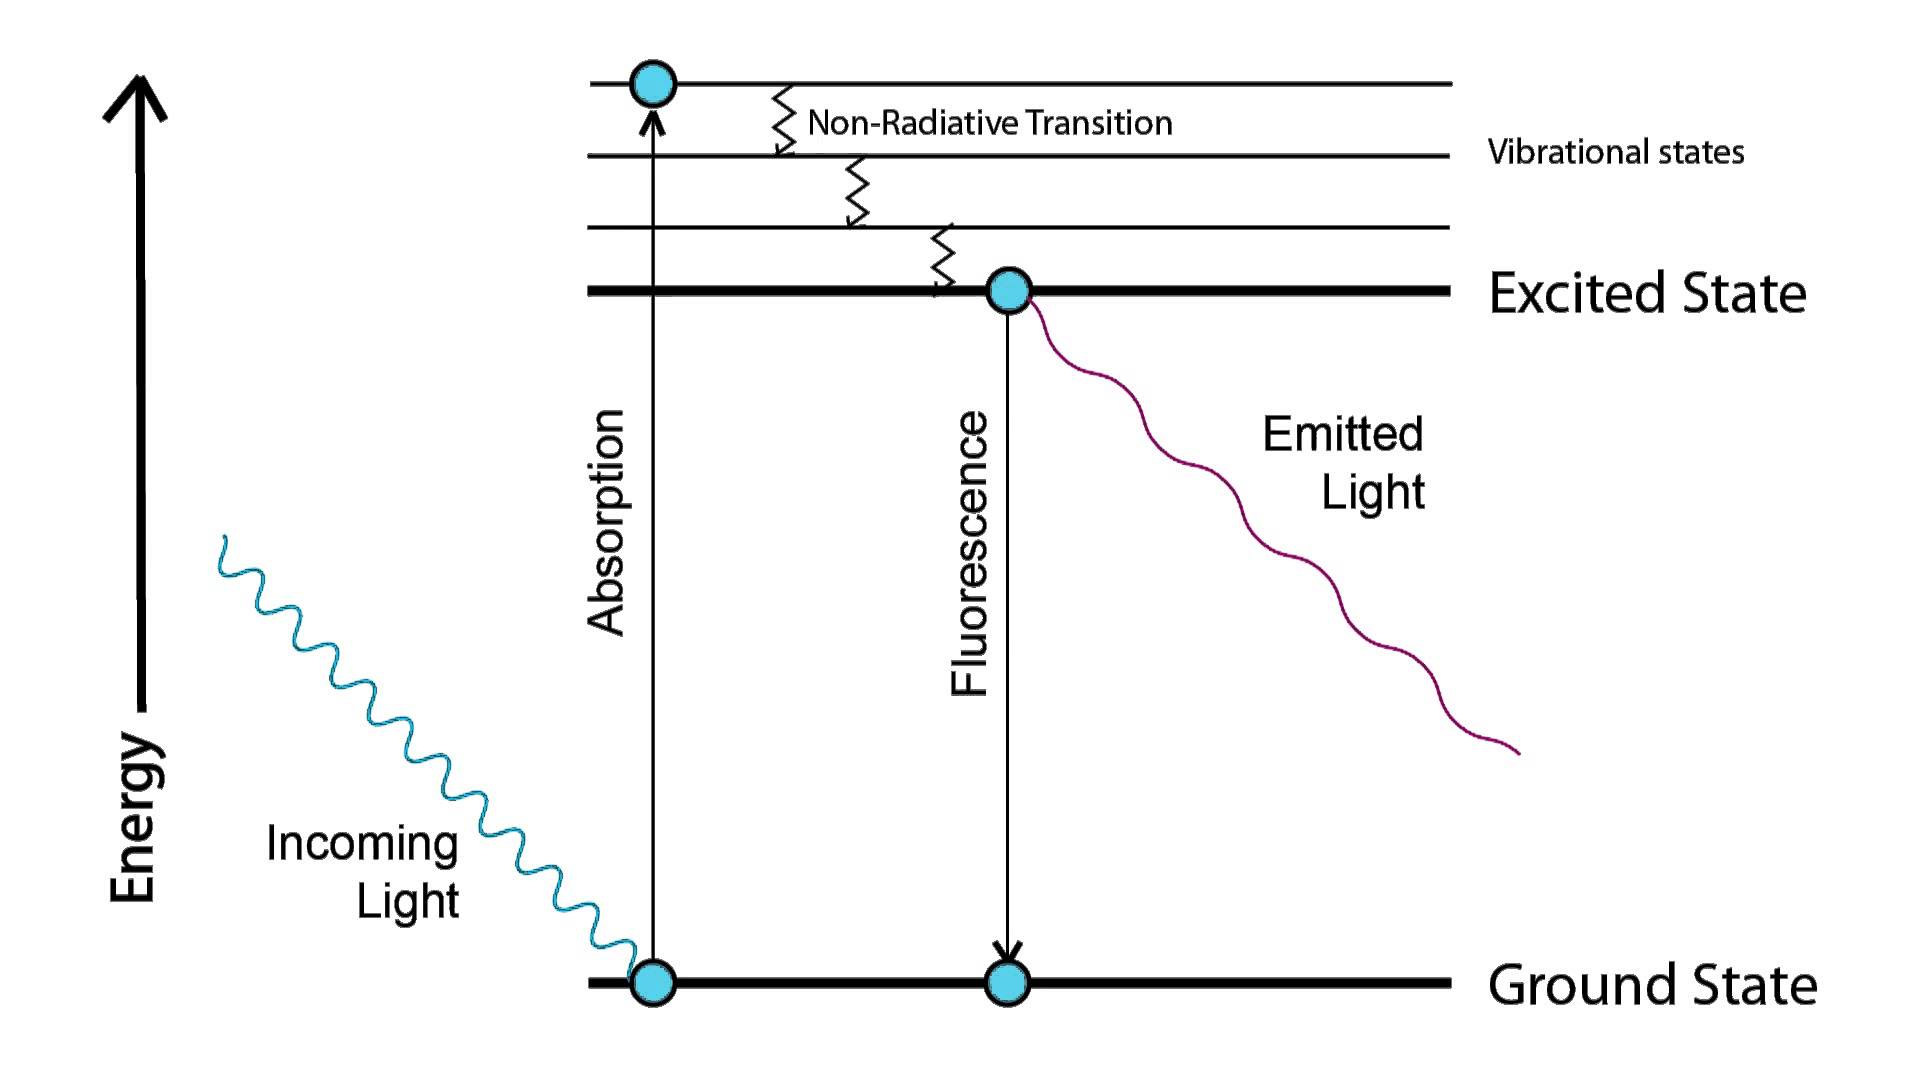
\includegraphics[width=1\linewidth]{/home/travis/build/rorynolan/phdthesis/img/Jablonski} \hfill{}

\caption{Jablonski diagram of the process of
fluorescence. Absorption causes excitation, relaxation causes the
emission of light.}\label{fig:Jablonski}
\end{figure}

\BeginKnitrBlock{definition}
\protect\hypertarget{def:unnamed-chunk-2}{}{\label{def:unnamed-chunk-2} }The
\emph{fluorescence lifetime} of an electron is the amount of time it
remains in the excited state before returning to the ground state.
\EndKnitrBlock{definition}

\BeginKnitrBlock{definition}
\protect\hypertarget{def:unnamed-chunk-3}{}{\label{def:unnamed-chunk-3} }A
\emph{fluorophore} is a fluorescent chemical compound that can re-emit
light upon light excitation.
\EndKnitrBlock{definition}

Fluorophores under constant excitation emit light one photon at a time
according to Poisson statistics.

\subsection{Phosphorescence}\label{phosphorescence}

\BeginKnitrBlock{definition}
\protect\hypertarget{def:unnamed-chunk-4}{}{\label{def:unnamed-chunk-4}
}Excited electrons can undergo a \emph{forbidden} transition into the
\emph{triplet} state T\textsubscript{1}, where they remain for a period
of milliseconds before relaxing to the ground state with the emission of
a photon. This is \emph{phosphorescence}.
\EndKnitrBlock{definition}

\subsection{Photobleaching}\label{photobleaching}

In reality, an incident photon can \emph{break} the fluorophore such
that it is unable to emit light. A fluorophore to which this has
happened is said to be \emph{photobleached}.

\section{Confocal light microscopy}\label{confocal-light-microscopy}

All of the images used in my PhD were collected on a confocal
microscope. This type of microscope guarantees that only in-focus light
is collected at the detector. See figure \ref{fig:confocal}.





\begin{figure}

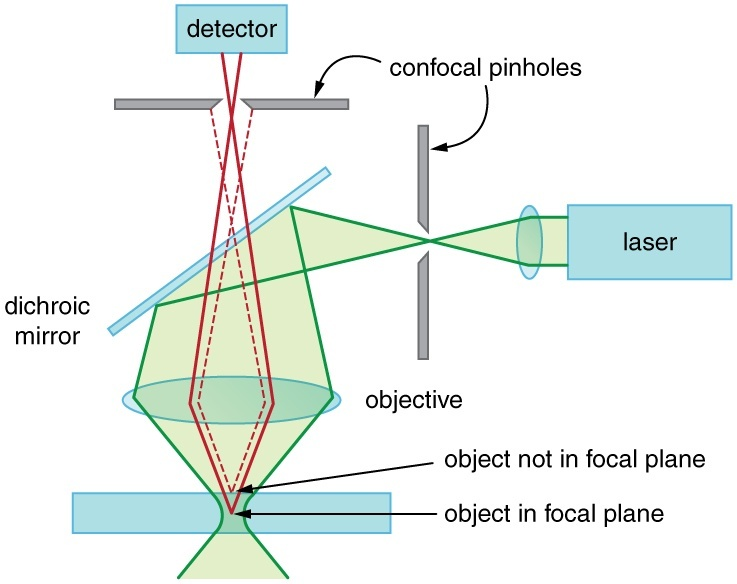
\includegraphics[width=0.7\linewidth]{/home/travis/build/rorynolan/phdthesis/img/quora_confocal} \hfill{}

\caption{Confocal microscope light path showing how out of
focus light does not make it to the detector.\footnote{Image courtesy of
  Quora: \url{https://www.quora.com/How-does-confocal-microscopy-work}}}\label{fig:confocal}
\end{figure}

\BeginKnitrBlock{definition}
\protect\hypertarget{def:unnamed-chunk-5}{}{\label{def:unnamed-chunk-5} }The
\emph{confocal volume} is the \emph{in-focus} volume within a sample
that is efficiently detected using a system designed with confocal
optics.\footnote{Definition from
  \url{http://www.fcsxpert.com/classroom/theory/what-is-confocal-volume.html}.}
\EndKnitrBlock{definition}

An image is acquired on a confocal microscope by scanning this apparatus
across a sample, collecting one pixel at a time.

\subsection{Detectors}\label{detectors}

There are many types of confocal microscope detector. I will discuss the
most common ones here. Most rely on the photoelectric effect
\citep{photoelectric}, a phenomenon whereby incident light upon a
certain material causes electrons to dissociate from that material.

\BeginKnitrBlock{definition}
\protect\hypertarget{def:unnamed-chunk-6}{}{\label{def:unnamed-chunk-6} }The
quantum efficiency of a detector is the fraction of fluorescent signal
that is reported by the detector.
\EndKnitrBlock{definition}

The quantum nature of the photoelectric effect makes it practically
impossible for detectors to reach 100\% efficiency.

\subsubsection{Photon multiplier tubes}\label{photon-multiplier-tubes}

Photon multiplier tubes (PMTs) use the photoelectric effect. Dissociated
electrons are accelerated through a potential difference towards a
cathode where their accumulated kinetic energy is used to to release
more electrons. These are then accelerated in vacuum towards another
cathode and so on for a predefined number of these accelerations until
at last the electrons are discharged into an anode where the current is
measured {[}HammamatsuPMT{]}. See figure \ref{fig:PMT}. This current
should correspond to the incident light intensity.






\begin{figure}

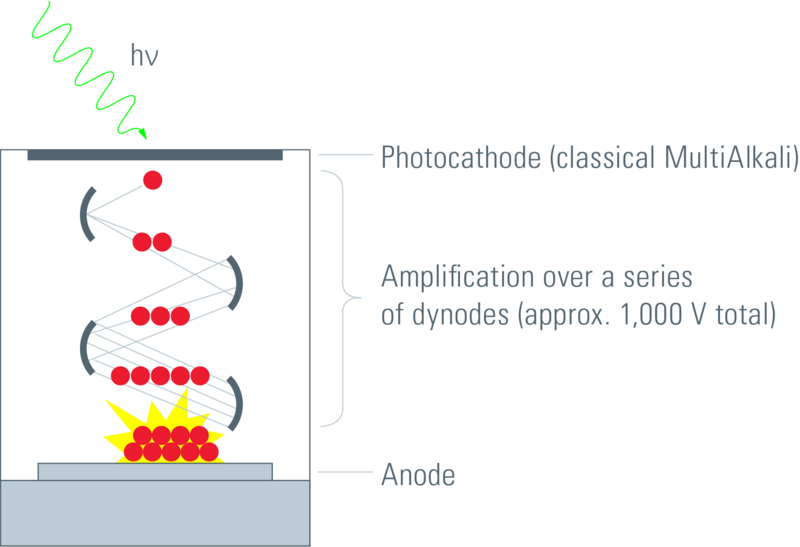
\includegraphics[width=1\linewidth]{/home/travis/build/rorynolan/phdthesis/img/PMT} \hfill{}

\caption{PMT detector setup. Electrons are dissociated by
photons at the photocathode, accelerated towards various other cathodes
where more and more are freed and then finally they arrive at the anode
where the current is measured \citep{LeicaDetectors}.}\label{fig:PMT}
\end{figure}

The quantum efficiency of standard PMTs is approximately 25\% for
blue-green light. This is because many incident photons on the
multi-alkali material of regular PMT photocathodes fail to free any
electrons. This problem gets worse at higher wavelengths where photons
have lower energy. PMTs also suffer significantly from thermal noise
(whereby dissociated electrons are created due to heat energy).

\subsubsection{Avalanche photo-diodes}\label{avalanche-photo-diodes}

\BeginKnitrBlock{definition}
\protect\hypertarget{def:unnamed-chunk-7}{}{\label{def:unnamed-chunk-7}
}\emph{Avalanche multiplication} in semiconductors occurs when free
electrons which are moving in an electric field across the semiconductor
collide with bound electrons, freeing them to move and indeed to free
more bound electrons. This compounding increase in free electrons in the
electric field leads to an increase in the electric current.
\EndKnitrBlock{definition}

Avalanche photo-diodes (APDs) are semiconductors that exploit the
photoelectric effect together with avalanche multiplication (the
photoelectric effect starts the avalanche) to convert light into
measurable electric current. See figure \ref{fig:APD}. They are somewhat
analogous to PMTs, using the avalanche effect in place of the series of
cathodes.





\begin{figure}

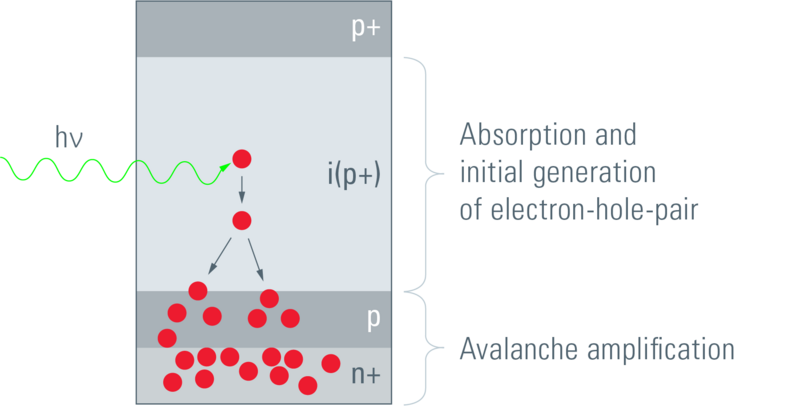
\includegraphics[width=1\linewidth]{/home/travis/build/rorynolan/phdthesis/img/APD} \hfill{}

\caption{APD detector setup. The incident photon dissociates an
electron. Given the electric field across the semiconductor this
electron is accelerated, initiating an avalanche \citep{LeicaDetectors}.}\label{fig:APD}
\end{figure}

The quantum efficiency of APDs can be as high as 45\%, however their
dynamic range is low and they can only function with low-intensity
light. APDs are less prone to thermal noise than PMTs.

\subsubsection{Hybrid detectors}\label{HyDs}

APDs have better sensitivity and lower noise, however PMTs have a larger
dynamic range. Hybrid detectors (HyDs) PMT and APD technology is
combined to get the best of both worlds. With HyDs, photons are
converted to electrons at the photocathode, then accelerated in vacuum
towards a semiconductor where they initiate an electron avalanche. See
figure \ref{fig:HyD}. The difference between HyDs and APDs is this
acceleration step.






\begin{figure}

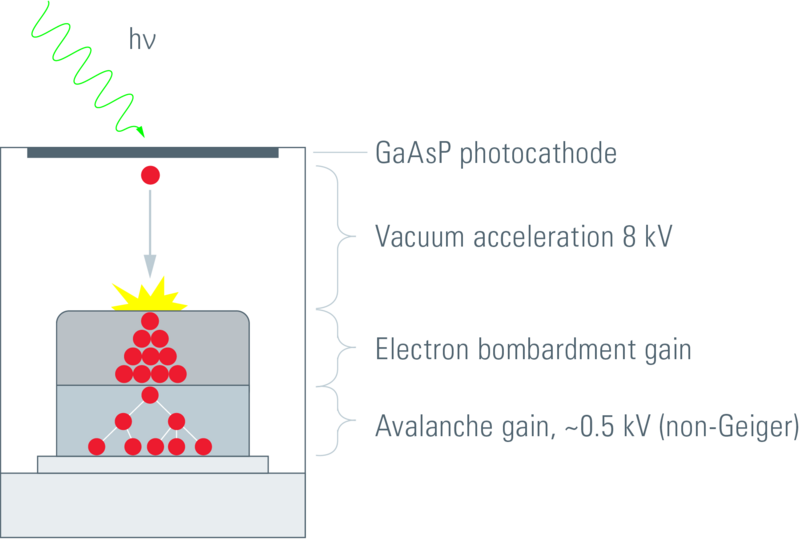
\includegraphics[width=1\linewidth]{/home/travis/build/rorynolan/phdthesis/img/HyD} \hfill{}

\caption{HyD detector setup. A photon dissociates an electron
from the photocathode, this electron is then accelerated PMT-style
towards an APD-style semiconductor setup, triggering an avalanche
\citep{LeicaDetectors}.}\label{fig:HyD}
\end{figure}

HyDs with GaAsP photocathodes achieve a quantum efficiency of up to
50\%. They also suffer least from detector afterpulsing, a phenomenon
which can cause real signal pulses to be followed by a feedback pulse at
a later time \citep{afterpulsing}.

With their superior sensitivity and dynamic range and low noise, HyDs
can be calibrated to enable \emph{photon-counting} mode whereby the
readout is in units of photons (not electron current). This is a much
more physically relevant readout, given that we are interested in
measuring fluorescence, which is very convenient for many biological
applications, not least fluorescence fluctuation spectroscopy (FFS,
discussed in section \ref{FFS}).

\BeginKnitrBlock{remark}
\iffalse{} {Remark. } \fi{}Henceforth, intensity counts will be assumed
to be in units of photons.
\EndKnitrBlock{remark}

\section{Widefield light microscopy}\label{widefield-light-microscopy}

With widefield microscopy, the entire sample is illuminated
simultaneously and the image is acquired by a camera. See figure
\ref{fig:widefield}. One advantage of this is the general simplicity of
the setup: the optics are less complex and there is no need for scanning
across the sample to acquire each pixel (which requires precise
robotics). Another example is that images can be acquired faster because
all pixels in a frame are acquired in parallel. The disadvantage of this
is that the absence of confocal optics means that out of focus light can
make it to the detection device (camera).





\begin{figure}

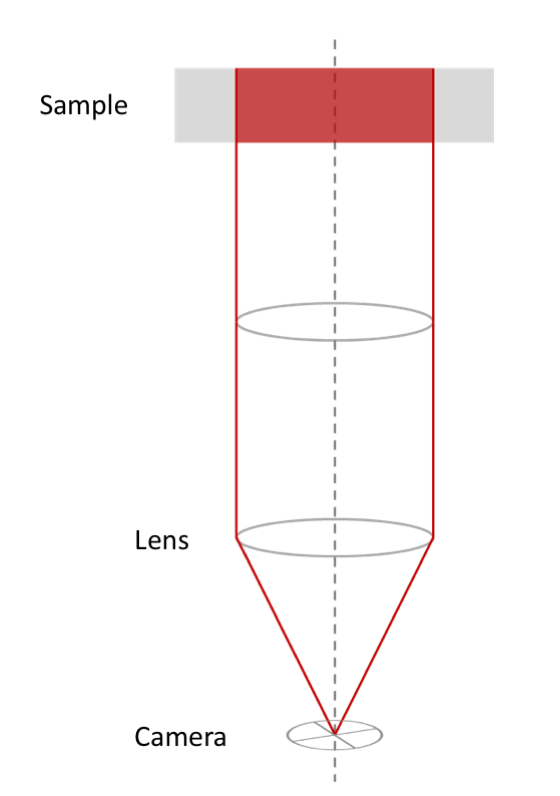
\includegraphics[width=0.5\linewidth]{/home/travis/build/rorynolan/phdthesis/img/Widefield} \hfill{}

\caption{Light travels from the uniformly illuminated
sample through a lens (or a few lenses) to the camera. Not the
simplicity of this setup relative to that of a confocal microscope.}\label{fig:widefield}
\end{figure}

\subsection{Total internal reflection
microscopy}\label{total-internal-reflection-microscopy}

\emph{Total internal reflection microscopy} (TIRF) uses the fact that
when total internal reflection (TIR) is occurring, an evanescent wave is
produced at the media boundary, but this evanescent wave is only present
very close to the boundary. See figure \ref{fig:TIRFig} \citep{TIRFig}.
The huge advantage of TIRF is that only a single plane is illuminated,
so when focusing on that plane, only in-focus light is collected
(because only the in-focus plane is illuminated). The main disadvantage
is that it is not applicable when one cannot get the object of interest
right at the cover slip. Looking at figure \ref{fig:TIRFig}, it is
evident that TIRF would be ideal for imaging the membrane but useless
for imaging the nucleus.





\begin{figure}

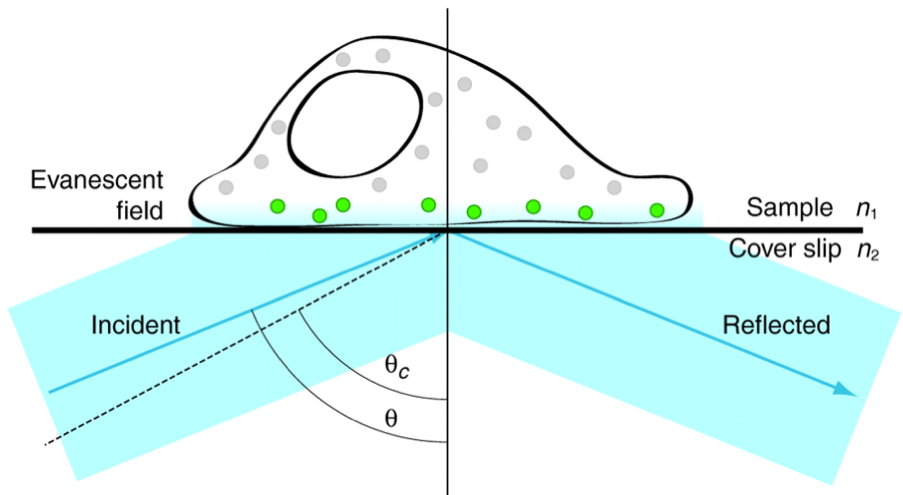
\includegraphics[width=1\linewidth]{/home/travis/build/rorynolan/phdthesis/img/TIRFig} \hfill{}

\caption{The thin evanescent wave close to the boundary
(between the cover slip and sample) where TIR is occurring. Only the
part of the sample within this thin evanescent wave is illuminated.}\label{fig:TIRFig}
\end{figure}

\subsection{Cameras}\label{cameras}

There are many types of camera available for widefield microscopes, the
most common being EMCCD, CMOS, and sCMOS cameras.

\subsubsection{EMCCD cameras}\label{emccd-cameras}

A charge-coupled device (CCD) is a device for the movement of electric
charge. An EMCCD camera is an array of CCDs (one per pixel). When
photons strike a CCD in the camera, electrons are dissociated by the
photoelectric effect. These free charges are then moved across the CCD
and this current can be measured and used as a measure of light
intensity (in arbitrary units) \citep{EMCCD}. The EM stands for
\emph{electron multiplied} which tells us that EMCCD cameras use an
amplification technique, just like PMTs and APDs (section
\ref{detectors}).

\subsubsection{CMOS cameras}\label{cmos-cameras}

Complementary metal--oxide--semiconductor cameras are arrays of
semiconductors (one per pixel), again utilizing the photoelectric effect
and the electric field across a semiconductor. CMOS cameras have
amplification for each pixel, whereas EMCCDs only have a few amplifiers
per camera \citep{CMOS}. This makes CMOS cameras more sensitive.

\subsubsection{sCMOS cameras}\label{scmos-cameras}

Scientific CMOS (sCMOS) cameras consist of a CMOS circuit bonded to a
CCD imaging substrate. These relatively new cameras offer very low
noise, rapid frame rates, large dynamic range, high resolution and wide
field of view, all cheaper than a regular CCD \citep{sCMOS}. sCMOS
cameras appear to better than anything that has come before.

\subsubsection{Being quantitative with
cameras}\label{being-quantitative-with-cameras}

For electronic reasons, the noise from certain pixels on all of the
cameras above may be correlated. This hinders some techniques in the
fluorescence correlation spectroscopy (section \ref{FCS}). However, with
careful characterization of the camera and correct mathematical
treatment, quantitative studies can be carried out with cameras. Indeed,
our group quantified the oligomeric state of the dynamin-2 protein at
the HIV-1 fusion pore using data from a TIRF microscope with an EMCCD
camera \citep{DanDynamin}.

\section{Intensity traces}\label{intensity-traces}

\BeginKnitrBlock{definition}
\protect\hypertarget{def:unnamed-chunk-9}{}{\label{def:unnamed-chunk-9} }A
\emph{fluorophore} is a fluorescent chemical compound that can re-emit
light upon light excitation.
\EndKnitrBlock{definition}

Consider figure \ref{fig:confocal-volume-particle}. A fluorophore enters
the confocal volume, is excited there and emits photons which are
collected by the detector. When the fluorophore is not in the confocal
volume (start and end), no photons are detected. When the particle is in
the confocal volume, photons it emits are collected at the detector.
Different numbers of photons are collected per unit time (per ms here).





\begin{figure}

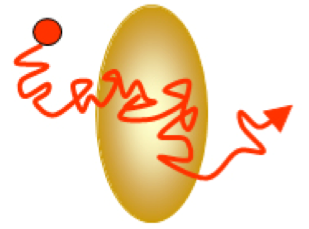
\includegraphics[width=0.5\linewidth]{/home/travis/build/rorynolan/phdthesis/img/confocal_volume_particle} 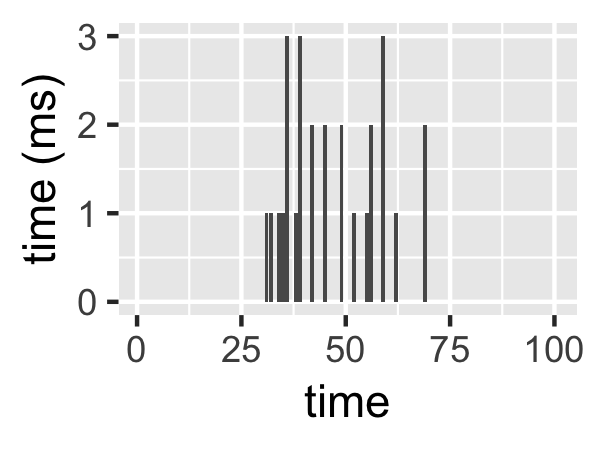
\includegraphics[width=0.5\linewidth]{/home/travis/build/rorynolan/phdthesis/img/cvp} \hfill{}

\caption{Left: a fluorophore diffusing
through the confocal volume. Right: the intensity trace due to this
fluorophore.}\label{fig:confocal-volume-particle}
\end{figure}

\BeginKnitrBlock{definition}
\protect\hypertarget{def:unnamed-chunk-10}{}{\label{def:unnamed-chunk-10}
}The time-series of intensity counts in a given pixel or image is
referred to as its \emph{intensity trace}.
\EndKnitrBlock{definition}

\section{Diffusion}\label{diffusion}

\BeginKnitrBlock{definition}
\protect\hypertarget{def:unnamed-chunk-11}{}{\label{def:unnamed-chunk-11}
}\emph{Diffusion} is the net movement of molecules or atoms from a
region of high concentration (or high chemical potential) to a region of
low concentration (or low chemical potential) as a result of random
motion of the molecules or atoms.
\EndKnitrBlock{definition}

Fick's first law of diffusion relates the concentration to the diffusive
flux, assuming a steady state. It describes how the flux goes from high
to low concentration areas, with magnitude proportional to the
concentration gradient. The law is:

\begin{equation}
J = -D\frac{d\varphi}{dx}
\label{eq:ficksfirst}
\end{equation}

where

\begin{itemize}
\tightlist
\item
  \(J\) is the diffusive flux
\item
  \(D\) is the diffusion constant
\item
  \(x\) is the position in space
\item
  \(\varphi\) is the concentration at position \(x\).
\end{itemize}

\BeginKnitrBlock{definition}
\protect\hypertarget{def:unnamed-chunk-12}{}{\label{def:unnamed-chunk-12}
}\emph{Brownian motion} is the random motion of particles suspended in a
fluid resulting from their collision with the fast-moving molecules in
the fluid \citep{Brownian}.
\EndKnitrBlock{definition}

\BeginKnitrBlock{definition}
\protect\hypertarget{def:unnamed-chunk-13}{}{\label{def:unnamed-chunk-13}
}In an ensemble of \(N\) particles, each of which occupies position
\(x_i(t)\) at time \(t\), the \emph{mean squared displacement} of the
particles in the ensemble is

\begin{equation}
\text{msd}(t) = \frac{1}{N}\sum_{i = 1}^N [x_i(t) - x_i(0)]^2
\label{eq:msd}
\end{equation}
\EndKnitrBlock{definition}

For free Brownian motion in 1 dimension, the expected value of the MSD
is \(\text{msd}(t) = 2Dt\), where \(D\) is the diffusion constant. For
free Brownian motion in \(d\) dimensions, the expected value of the MSD
is \(\text{msd}(t) = 2dDt\), reflecting the fact that free Brownian
motion in \(d\) dimensions is one-dimensional free Brownian motion
happening simultaneously and independently in each individual dimension.

These definitions are the formally correct ones. In biophysics, however,
both of these processes (diffusion and Brownian motion) are most often
referred to as \emph{diffusion}. Usually, in biophysics one is
interested in proteins which move around in a medium like the cytoplasm
or the cell membrane. When this is referred to as \emph{diffusion}, it
is what is defined as Brownian motion above. Henceforth when I use the
term \emph{diffusion}, this Brownian motion type of movement can be
assumed.

\subsection{Anomalous diffusion}\label{anomalous-diffusion}

\emph{Anomalous diffusion} is a diffusion process whereby equation
\eqref{eq:MSD} no longer holds and the relationship between MSD and time
becomes non-linear. Knowing whether diffusion is anomalous or free can
offer biological insight. For example, regions of free and anomalous
diffusion were measured with FCS (section \ref{FCS}) to investigate the
spatiotemporal heterogeneity of lipid interaction in the plasma membrane
of living cells \citep{EggSTEDFCS}. The pair correlation function
approach (section \ref{PCF})

\section{Fluorescence fluctuation spectroscopy}\label{FFS}

Broadly, fluorescence fluctuation spectroscopy (FFS) is the analysis of
the intensity fluctuation of a fluorescence signal \citep{FFS}. This
very often takes the form of moment analysis \citep{QianElson}. Briefly,
moment analysis is an attempt to extract data from a distribution of
values using its \emph{moments}. The first moment of a distribution is
its mean value, the second moment is its variance. The
\(n\)\textsuperscript{th} moment of a random \(X\) with expected value
\(E[X]=\mu\) for \(n>1\) is \(E[(X - \mu)^n]\).

Intensity traces can be viewed as distributions with moments. For
example, the intensity trace in figure
\ref{fig:confocal-volume-particle} has mean 0.35 and variance 0.69.

\subsection{Number and brightness}\label{number-and-brightness}

\emph{Number and brightness} (N\&B, \citet{NB}) is an FFS technique for
quantifying the oligomeric states of fluorescently labelled proteins.
What follows is a mathematical description of the technique.

\BeginKnitrBlock{definition}
\protect\hypertarget{def:unnamed-chunk-14}{}{\label{def:unnamed-chunk-14}
}An \emph{entity} is a set of molecules which are chemically bound.
\EndKnitrBlock{definition}

\BeginKnitrBlock{definition}
\protect\hypertarget{def:unnamed-chunk-15}{}{\label{def:unnamed-chunk-15}
}The brightness \(\epsilon\) of an entity is the mean number of photon
detector counts it gives per unit time when in the illumination
(confocal) volume.
\EndKnitrBlock{definition} For an image series where the
\(i\)\textsuperscript{th} slice in the stack is the image acquired at
time \(t = i\), for a given pixel position \((x, y)\), we define
\(\langle I \rangle\) as the mean intensity of that pixel over the image
series and \(\sigma^2\) as the variance in that intensity. Define \(n\)
as the mean number of entities in the illumination volume corresponding
to that pixel. Assuming that all entities are mobile, we have

\begin{align}
N &= \frac{\langle I \rangle^2}{\sigma^2} = \frac{\epsilon n}{1 + \epsilon} \label{eq:NB1-1} \\
B &= \frac{\sigma^2}{\langle I \rangle} = 1 + \epsilon \label{eq:NB1-2}
\end{align}

where \(N\) and \(B\) are referred to as the \emph{apparent number} and
\emph{apparent brightness} respectively. This gives

\begin{align}
\epsilon &= \frac{\sigma^2}{\langle I \rangle} - 1 \label{eq:NB2-1} \\
n &= \frac{\langle I \rangle^2}{\sigma^2 - \langle I \rangle} \label{eq:NB2-2}
\end{align}

\begin{quote}
--- \citet{NBreview}\footnote{This is a formulation of N\&B that I wrote
  in a 2017 review of the technique.}
\end{quote}

The quantity \(\epsilon\) is a relative measure of oligomeric state.
That is, \(\epsilon\) will be twice as big for dimers as it is for
monomers, three times as big for trimers as it is for monomers and so
on.

The way that N\&B experiments to determine unknown oligomeric states are
generally done is as follows:

\begin{enumerate}
\def\labelenumi{\arabic{enumi}.}
\tightlist
\item
  For a given laser power and fluorophore with a system where all
  entities are known to be monomeric, measure the brightness
  \(\epsilon\). Call this \(\epsilon_\text{monomer}\).
\item
  With the same laser power and fluorophore but now with a system where
  the oligomeric state is unknown, measure the brightness \(\epsilon\)
  again. Call this \(\epsilon_\text{unknown}\).
\item
  The unknown oligomeric state is equal to
  \(\epsilon_\text{unknown} / \epsilon_\text{monomer}\).
\end{enumerate}

Number and brightness has specific pixel dwell-time and frame rate
requirements. These were first articulated in my 2017 review of N\&B
\citep{NBreview}.

\BeginKnitrBlock{definition}
\protect\hypertarget{def:unnamed-chunk-16}{}{\label{def:unnamed-chunk-16}
}The \emph{pixel dwell time} \(t_\text{dwell}\) of a scanning confocal
microscope is the amount of time it spends collecting photons at each
given pixel before moving on to the next pixel.
\EndKnitrBlock{definition}

It is essential that the pixel dwell time is the same for each pixel,
particularly for FFS. This is something that must be carefully verified
on each instrument.

\BeginKnitrBlock{definition}
\protect\hypertarget{def:unnamed-chunk-17}{}{\label{def:unnamed-chunk-17}
}The \emph{frame time} of a scanning confocal microscope is the amount
of time it takes to acquire the data for all of the pixels in a whole
frame. That is the length of time from the start of detectionion of
photons from the first pixel to the end of detection of photons from the
last pixel.
\EndKnitrBlock{definition}

\BeginKnitrBlock{definition}
\protect\hypertarget{def:unnamed-chunk-18}{}{\label{def:unnamed-chunk-18}
}The mean \emph{residence time} \(\tau_D\) of a particle in the confocal
volume is the average length of time that a particle that enters the
confocal volume resides in that volume before exiting.
\EndKnitrBlock{definition}

The requirement is \(t_\text{dwell} \ll \tau_D \ll t_\text{frame}\).
This ensures that:

\begin{enumerate}
\def\labelenumi{\arabic{enumi}.}
\tightlist
\item
  When acquiring photons at a given pixel, the underlying configuration
  of entities is constant (there's not enough time for the entities to
  move and change their configuration).
\item
  When the scanner returns to a given pixel (one frame time later), the
  underlying configuration has changed totally since the last time the
  scanner was at this pixel (because so much time has passed, all of the
  diffusing entities have moved a lot in the meantime).
\end{enumerate}

Both of these points are implicitly assumed in the derivation of the
N\&B equations so it is essential to get these acquisition parameters
right. This is discussed at length in \citet{NBreview}.

An important property of N\&B is that if all fluorescent particles are
immobile, then \(B = 1\). This is because photon emission from
stationary sources happens according to a Poisson distribution. Poisson
distributions have variance equal to mean, this implies \(\sigma^2\) =
\(\langle I \rangle\) which gives
\(B = \frac{\sigma^2}{\langle I \rangle} = 1\).

The N\&B technique is fraught with technical difficulties. Principal of
these is the problem of photobleaching. Most of my PhD focused on
corrections for photobleaching. This is discussed in chapter
\ref{photobleaching-correction}.

\section{Fluorescence correlation spectroscopy}\label{FCS}

Fluorescence correlation spectroscopy (FCS) is the correlation analysis
of fluorescence intensity fluctuations. For this reason, FCS can be
described as a subfield of FFS \citep{FFSnewage}. In practice, FFS is
mostly used to refer to the non-FCS parts of the whole FFS field. I will
follow that convention.

First, let us introduce some concepts from statistics.

\BeginKnitrBlock{definition}[statistics]
\protect\hypertarget{def:unnamed-chunk-19}{}{\label{def:unnamed-chunk-19}
\iffalse (statistics) \fi{} }The \emph{correlation} between two random
variables \(X\) and \(Y\) with expected values \(\mu_X\) and \(\mu_Y\)
and standard deviations \(\sigma_X\) and \(\sigma_Y\) is

\begin{equation}
\text{corr}(X, Y) = \frac{E[(X - \mu_X)(Y - \mu_Y)]}{\sigma_X \sigma_Y}
\label{eq:correlation}
\end{equation}

where \(E\) is the expectation operator.
\EndKnitrBlock{definition}

\BeginKnitrBlock{definition}[statistics]
\protect\hypertarget{def:unnamed-chunk-20}{}{\label{def:unnamed-chunk-20}
\iffalse (statistics) \fi{} }\emph{Autocorrelation} \(G(X; \tau)\), is
the correlation of a signal \(X\) with a delayed copy of itself as a
function of the delay \(\tau\).

\begin{equation}
G(X; \tau) = \text{corr}(X_t, X_{t + \tau}) = \frac{E[(X_t - \mu_X)(X_{t + \tau} - \mu_X)]}{\sigma^2_X}
\label{eq:autocorrelation}
\end{equation}
\EndKnitrBlock{definition}

\BeginKnitrBlock{definition}[statistics]
\protect\hypertarget{def:unnamed-chunk-21}{}{\label{def:unnamed-chunk-21}
\iffalse (statistics) \fi{} }The \emph{cross-correlation} of two series
is the correlation of one with a delayed copy of the other as a function
of the delay.

\begin{equation}
\text{crosscorr}(X, Y; \tau) = \text{corr}(X_t, Y_{t + \tau}) = \frac{E[(X_t - \mu_X)(Y_{t + \tau} - \mu_Y)]}{\sigma_X \sigma_Y}
\label{eq:crosscorrelation}
\end{equation}
\EndKnitrBlock{definition}

For the purposes of FCS, these quantities were redefined as follows.

\BeginKnitrBlock{definition}[FCS]
\protect\hypertarget{def:unnamed-chunk-22}{}{\label{def:unnamed-chunk-22}
\iffalse (FCS) \fi{} }The \emph{correlation} between two random
variables \(X\) and \(Y\) with expected values \(\mu_X\) and \(\mu_Y\)
and standard deviations \(\sigma_X\) and \(\sigma_Y\) is

\begin{equation}
\text{corr}(X, Y) = \frac{E[(X - \mu_X)(Y - \mu_Y)]}{\mu_X \mu_Y}
\label{eq:FCScorrelation}
\end{equation}

where \(E\) is the expectation operator.
\EndKnitrBlock{definition}

\BeginKnitrBlock{definition}[FCS]
\protect\hypertarget{def:unnamed-chunk-23}{}{\label{def:unnamed-chunk-23}
\iffalse (FCS) \fi{} }\emph{Autocorrelation} \(G(X; \tau)\), is the
correlation of a signal \(X\) with a delayed copy of itself as a
function of the delay \(\tau\).

\begin{equation}
G(X; \tau) = \text{corr}(X_t, X_{t + \tau}) = \frac{E[(X_t - \mu_X)(X_{t + \tau} - \mu_X)]}{\mu^2_X}
\label{eq:FCSautocorrelation}
\end{equation}
\EndKnitrBlock{definition}

\BeginKnitrBlock{definition}[FCS]
\protect\hypertarget{def:unnamed-chunk-24}{}{\label{def:unnamed-chunk-24}
\iffalse (FCS) \fi{} }The \emph{cross-correlation} of two series is the
correlation of one with a delayed copy of the other as a function of the
delay.

\begin{equation}
\text{crosscorr}(X, Y; \tau) = \text{corr}(X_t, Y_{t + \tau}) = \frac{E[(X_t - \mu_X)(Y_{t + \tau} - \mu_Y)]}{\mu_X \mu_Y}
\label{eq:FCScrosscorrelation}
\end{equation}
\EndKnitrBlock{definition}

The reason for these redefinitions (which just involve replacing
standard deviations with means in the denominators of each expression)
is that with the FCS definition, the autocorrelation has the nice
property that for normal diffusion

\begin{equation}
G(X; 0) = \frac{1}{n}
\label{eq:FCSautocorrprop}
\end{equation}

where \(n\) is the mean number of fluorescent particles in the focal
volume. The convenience of the statistics definitions is that there,
correlations are guaranteed to be in \([-1, 1]\), with \(0\)
representing no correlation, \(1\) perfect positive correlation and
\(-1\) perfect negative correlation; this is lost with the FCS
definitions: 0 still represents no correlation, but correlation values
are no longer bounded, so the ideas of perfect correlation are lost.

I felt it necessary to provide these definitions for two reasons:

\begin{enumerate}
\def\labelenumi{\arabic{enumi}.}
\tightlist
\item
  It is important for people from the fields of FCS and pure
  mathematics/statistics to know that they have different definitions
  for the same thing.
\item
  In FCS, it's very common for people to mistake correlation for
  cross-correlation. This is unfortunate, but knowing about this common
  mistake is essential for navigating the field in a sensible manner. It
  seems that when people in the FCS field correlate the signals from two
  separate channels, they use the term \emph{cross}-correlation, even
  though they're only using correlation. I think the idea of working
  \emph{across} two or more channels (and ideas such as
  \emph{cross}-talk) leads to this confusion.
\end{enumerate}

\BeginKnitrBlock{remark}
\iffalse{} {Remark. } \fi{}Henceforth, the FCS defintions of these
quantities will be assumed.
\EndKnitrBlock{remark}

\subsection{Correlation}\label{correlation}

Suppose that two proteins of interest A and B are labelled with red and
green fluorophores respectively (and there is no bleed-through between
these red and green channels).

If these proteins are interacting, then

\begin{itemize}
\tightlist
\item
  interaction implies that A and B \emph{co-diffuse}
\item
  this implies that A and B co-diffuse
\item
  this implies that for a given volume in the sample
\item
  more of A implies more of B
\item
  less of A implies less of B
\item
  more of B implies more of A
\item
  less of B implies less of A
\end{itemize}

Since the number of photons emitted is proportional to the amount of
fluorophores present, it follows that

\begin{itemize}
\tightlist
\item
  more red photons implies more green photons
\item
  less red photons implies less green photons
\item
  more green photons implies more red photons
\item
  less green photons implies less red photons
\end{itemize}

Altogether, this implies that the intensity traces from the red and
green channels will be correlated. If these proteins are not
interacting, then the intensity traces from the red and green channels
will not be correlated. Thus, interaction of red A and green B
necessarily leads to correlation in fluorescent signals from the red and
green channels.\footnote{This correlation may not always be detectable
  due to weak interaction or weak signal.}

\subsection{Autocorrelation}\label{autocorrelation}

As mentioned already, the autocorrelation function (ACF) can be used to
count the number of particles in the confocal volume. It can also be
used to measure diffusion coefficients for various types of diffusion
(normal, anomalous, polydisperse, etc.). The ACF is not used in my PhD.

\subsection{Cross-correlation}\label{cross-correlation}

The cross-correlation of intensity traces from nearby pixels can be used
to measure the velocity of the movement of the labelled particles
between these two pixels \citep{STICS}.

\subsubsection{Pair correlation function}\label{PCF}

The phrase \emph{pair correlation function}\footnote{This was needless,
  it could just be called \emph{cross-correlation function} (PCF) but
  for the confusion about the term \emph{cross-correlation} in the FCS
  field.} was coined for this idea of cross-correlating intensity traces
from nearby pixels. The PCF was used to image barriers to diffusion
\citep{PCF} using the idea that the spatiotemporal correlation caused by
particles moving from one place to another will not be present for
positions \(p_1\) and \(p_2\) if they are on opposite sides of a
barrier, because the barrier prevents travel from \(p_1\) to \(p_2\). It
has also been used to create \emph{diffusion tensors}: maps of diffusion
velocities at every pixel \citep{DiffusionTensor}; this approach is
similar to that of \citet{STICS}.

\subsection{Cross-correlated
brightness}\label{cross-correlated-brightness}

\emph{Cross-correlated brightness} \citep{ccNB} molds the correlation
idea (section \ref{correlation}) into the framework of N\&B. Suppose
there are two channels with intensities \(I_1\) and \(I_2\).

\BeginKnitrBlock{definition}[cross-variance]
\protect\hypertarget{def:unnamed-chunk-26}{}{\label{def:unnamed-chunk-26}
\iffalse (cross-variance) \fi{} }

\begin{equation}
\sigma^2_\text{cc} = E[(I_2 - \langle I_1 \rangle)(I_2 - \langle I_2 \rangle)]
\label{eq:cross-var}
\end{equation}
\EndKnitrBlock{definition}

\BeginKnitrBlock{definition}[cross-correlated brightness]
\protect\hypertarget{def:unnamed-chunk-27}{}{\label{def:unnamed-chunk-27}
\iffalse (cross-correlated brightness) \fi{} }

\begin{equation}
B_\text{cc} = \frac{\sigma^2_\text{cc}}{\sqrt{\langle I_1 \rangle \langle I_2 \rangle}}
\label{eq:cross-corr-nb}
\end{equation}
\EndKnitrBlock{definition}

\(B_\text{cc}\) is related to \(\text{corr}(I_1, I_2)\) by

\begin{equation}
B_\text{cc} = \sqrt{\langle I_1 \rangle \langle I_2 \rangle} \times \text{corr}(I_1, I_2)
\label{eq:bcc-corr}
\end{equation}

This means that \(B_\text{cc}\) is just a scaled version of correlation.
The need for this redefinition is unclear (but it is no harm). It does
make the formula look like the brightness formula \eqref{eq:NB1-2}, but no
such oligomeric state information can be gleaned from \(B_\text{cc}\).
It is merely useful as a relative measure of interaction: higher
\(B_\text{cc}\) means more interaction, lower \(B_\text{cc}\) means less
interaction. It is commonly used to identify interactions. Then,
conventional N\&B performed on each of the channels (1 and 2) can be
used to measure the stoichiometry of the interaction.

\BeginKnitrBlock{remark}
\iffalse{} {Remark. } \fi{}Since cross-correlated brightness uses
correlation but not cross-correlation, it is a prime example of the
confusing naming that pervades FCS. It should be called \emph{correlated
brightness}. Rather than rename it, I will continue to refer to it as
cross-correlated brightness.
\EndKnitrBlock{remark}

\section{Applications of FCS and FFS}\label{applications-of-fcs-and-ffs}

FCS and FFS have been used in thousands of research projects. Here I
number but a few for the sake of interest and to give biological context
to these techniques.

Number and brightness (the prominent imaging FFS technique) has been
used to:

\begin{itemize}
\tightlist
\item
  characterize the state of DNA aggregation in live cells
  \citep{Mieruszynski}
\item
  measure the stoichiometry of scaffold complexes in live neurons
  \citep{Moutin}
\item
  quantify interactions in gene expression networks \citep{Declerck}
\item
  measure the oligomeric state of the dynamin-2 protein at the HIV-1
  fusion pore \citep{DanDynamin}
\item
  measure the stoichiometry of the interaction of HIV-1 with its
  receptor and co-receptor over time in the pre-fusion process
  \citep{HIVstoichiometry}
\end{itemize}

FCS has been used to:

\begin{itemize}
\tightlist
\item
  reveal structural and functional properties of promyelocytic leukemia
  nuclear bodies \citep{Hoischen}
\item
  demonstrate that HIV-1 evades antibody-dependent phagocytosis
  \citep{Gach}
\item
  determine the size of nanodomains \citep{Fenz}
\item
  perform chromatographic measurements \citep{Kisley}
\item
  quantify interactions of membrane proteins \citep{Ly}
\end{itemize}

\chapter{Instrumentation and
Software}\label{instrumentation-and-software}

\section{Instrumentation}\label{instrumentation}

All of the images used in this thesis were acquired on a Leica SP8
confocal microscope\footnote{\url{https://www.Leica-microsystems.com/products/confocal-microscopes/details/product/Leica-tcs-sp8}}
equipped with hybrid detectors (section \ref{HyDs}). Importantly, the
detectors that we have on this microscope are capable of photon
counting.

\section{Software programs, languages and
tools}\label{software-programs-languages-and-tools}

\subsection{C++}\label{c}

\emph{C++} \citep{cpp} is a general-purpose programming language
optimized for performance (speed), efficiency (with use of computer
resources) and flexibility.\footnote{\url{https://en.wikipedia.org/wiki/C\%2B\%2B}}
I used it for its speed, since many of the algorithms that I developed
were quite computationally intensive and hence speed was an important
consideration.

\subsection{R}\label{r}

\emph{R} \citep{R} is a programming language and free software
environment for statistical computing and graphics.\footnote{\url{https://en.wikipedia.org/wiki/R_(programming_language)}}
I use R primarily as a wrapper for my C++ code to make my algorithms
more user-friendly. R is best used with the \emph{RStudio} integrated
development environment.\footnote{\url{https://www.rstudio.com}}

\hypertarget{imagej}{\subsection{ImageJ}\label{imagej}}

\emph{ImageJ} \protect\hyperlink{imagej}{ImageJ} is an open source image
processing program designed for scientific multidimensional
images.\footnote{\url{https://imagej.net}} It is the preferred image
viewing and analysis software in the community. I have written my
software in C++ and R because they are easier for developers, but I
still intend to translate my image-related algorithms ImageJ plugins.
ImageJ is best used via the FIJI \citep{FIJI} distribution.\footnote{\url{https://imagej.net/Fiji}}

\subsection{Git and GitHub}\label{git-and-github}

Git is a free and open source distributed version control system
designed to handle everything from small to very large projects with
speed and efficiency.\footnote{\url{https://git-scm.com/}} GitHub is a
web-based hosting service for version control using Git.\footnote{\url{https://en.wikipedia.org/wiki/GitHub}}
All of the computer code used during my thesis can be found on my GitHub
at \url{https://github.com/rorynolan}. The vast majority of my time
during my thesis was spent writing code so this GitHub account is the
best record of the work that I have done.

\section{My software packages}\label{my-software-packages}

\subsection{\texorpdfstring{\texttt{ijtiff}}{ijtiff}}\label{ijtiff}

An R package for general purpose TIFF file I/O. This is currently the
only such package with read and write support for TIFF files with
floating point (real-numbered) pixels, and the only package that can
correctly import TIFF files that were saved from \emph{ImageJ}
\citep{ImageJ}. R has millions of users worldwide so this TIFF I/O
capability is a basic need for masses of people. \texttt{ijtiff} gets
348 downloads per month which amounts to 2,479 since it was first
released.

This package is part of the \emph{rOpenSci} project. rOpenSci is a
non-profit initiative founded to make scientific data retrieval
reproducible.\footnote{\url{https://ropensci.org/about}} This package
was peer reviewed and published \citep{ijtiff}.

\subsection{\texorpdfstring{\texttt{autothresholdr}}{autothresholdr}}\label{autothresholdr}

\texttt{autothresholdr} provides the \emph{ImageJ} \citep{ImageJ}
\emph{Auto Threshold} plugin \citep{autothresholdr} functionality to R
users. It gets 643 downloads per month which amounts to 10,873 since it
was first released.

\subsection{\texorpdfstring{\texttt{detrendr}}{detrendr}}\label{detrendr}

\texttt{detrendr} is an R package for detrending images (correcting for
photobleaching). It provides all detrending algorithms mentioned in
section \ref{photobleaching-correction}. The detrending is done in C++
in the background for speed but it is wrapped in an R package for ease
of use. It gets 373 downloads per month which amounts to 3,349 since it
was first released.

\subsection{\texorpdfstring{\texttt{filesstrings}}{filesstrings}}\label{filesstrings}

\texttt{filesstrings} is an R package providing convenient functions for
moving files, deleting directories, and a variety of string operations
that facilitate manipulating file names and extracting information from
strings. The motivation for making this package was to facilitate the
use of file names for metadata. This is very common in microscopy,
e.g.~a file name like \texttt{well1\_cell1\_before\_drug\_addition.tif}
is often seen. Using file names for metadata like this is a good idea,
however if the naming or the extraction of data from these names is
inconsistent, analysis becomes a nightmare and less reproducible. This
package was peer reviewed and published \citep{filesstrings}. It gets
815 downloads per month which amounts to 13,818 since it was first
released.

\subsection{\texorpdfstring{\texttt{exampletestr}}{exampletestr}}\label{exampletestr}

\BeginKnitrBlock{definition}
\protect\hypertarget{def:unnamed-chunk-29}{}{\label{def:unnamed-chunk-29}
}\emph{Unit testing} is a software testing method by which individual
units of source code, sets of one or more computer program modules
together with associated control data, usage procedures, and operating
procedures, are tested to determine whether they are fit for
use.\footnote{\url{https://en.wikipedia.org/wiki/Unit_testing}}
\EndKnitrBlock{definition}

Unit testing is a tool to verify that software is performing as
intended. It is a great way to discover bugs in software.
\texttt{exampletestr} is an R package which makes it easier for R
package developers to write unit tests for their packages. It helped me
to eradicate many bugs in all of my packages. Interestingly,
\texttt{exampletestr} was used to unit test and eradicate bugs in
itself! This package was peer reviewed and published in
2017.\citep{exampletestr} It gets 521 downloads per month which amounts
to 8,441 since it was first released.

\subsection{\texorpdfstring{\texttt{brownded}}{brownded}}\label{brownded}

\texttt{brownded} is an R software package
(\url{https://github.com/rorynolan/brownded}) for simulating bounded
Brownian motion in any number of dimensions, where \emph{bounded}
Brownian motion is Brownian motion in an \(n\)-dimensional box where the
particles collide elastically (without loss of energy) with the
boundaries of the box. \texttt{brownded} allows specification of the
number of dimensions, the number of particles, the size of the box and
the diffusion coefficient of the particles.

\texttt{brownded} also facilitates the simulation of images created from
fluorescent particles undergoing bounded Brownian motion. It allows
specification of the time at which each image should be taken, the pixel
size and the brightness of the particles. Each fluorescent particle
contributes photon counts to its pixel of residence at that time
according to a Poisson process.

Finally, \texttt{brownded} facilitates the synthetic bleaching of
fluorescent particles so bleaching can be investigated with images
produced with \texttt{brownded}.

\chapter{Photobleaching Correction}\label{photobleaching-correction}

\section{Introduction to
photobleaching}\label{introduction-to-photobleaching}

In the ideal case, an \emph{incident} photon of appropriate wavelength
is absorbed by a fluorophore, promoting the fluorophore to an excited
state; subsequently, the fluorophore relaxes down to its ground state by
emitting a photon. In reality, it is possible that the incident photon
can \emph{break} the fluorophore with the result that it will no longer
emit light. This breaking is referred to as \emph{photobleaching} (or
\emph{bleaching} for short). Bleaching causes a diminution in the number
of effective fluorophores which is a direct cause of a loss of
fluorescent signal.

Many quantitative methods in fields such as fluorescence fluctuation
spectroscopy (FFS) and fluorescence correlation spectroscopy (FCS)
implicitly assume that there is no bleaching in the data. Hence, data
(image series) with significant levels of photobleaching must be
corrected prior to the application of equations and algorithms in these
fields. A main focus of this thesis is on how to correct fluorescent
image series for the effects of bleaching, given that bleaching
\emph{does} occur. There is no attempt to understand \emph{why} and/or
\emph{how} photobleaching occurs.

\BeginKnitrBlock{remark}
\iffalse{} {Remark. } \fi{}All of the current literature mentions
bleaching correction as being purely for correcting the problem of
non-stationary mean (NSM), neglecting the problem of non-stationary
variance (NSV). Figure \ref{fig:visualize-variance-decrease} shows that
NSM and NSV go hand-in-hand. Correction for NSM is referred to as trend
removal or \emph{detrending}. Hence, the terms \emph{detrending} and
\emph{bleaching correction} have come to be used interchangeably. I will
follow this convention and use the term \emph{detrending} from now on to
mean correction for NSM and possibly also NSV. Starting at section
\ref{exponential-fitting-detrending}, the focus is on correcting for
NSM. Discussion of correction for NSV starts in section
\ref{correcting-for-non-stationary-variance}.
\EndKnitrBlock{remark}

\section{The effects of bleaching in FCS and
FFS}\label{the-effects-of-bleaching-in-fcs-and-ffs}

We simulate two image series, each with 100,000 diffusing fluorescent
particles. In the first image series (\texttt{img1}), these have
brightness \(\epsilon = 4\) and in the second (\texttt{img2}) they have
brightness \(\epsilon = 7\). See figure \ref{fig:bleaching-sim}. We
bleach these by 15\% and 20\% to create \texttt{img1\_bleached} and
\texttt{img2\_bleached} respectively.






\begin{figure}

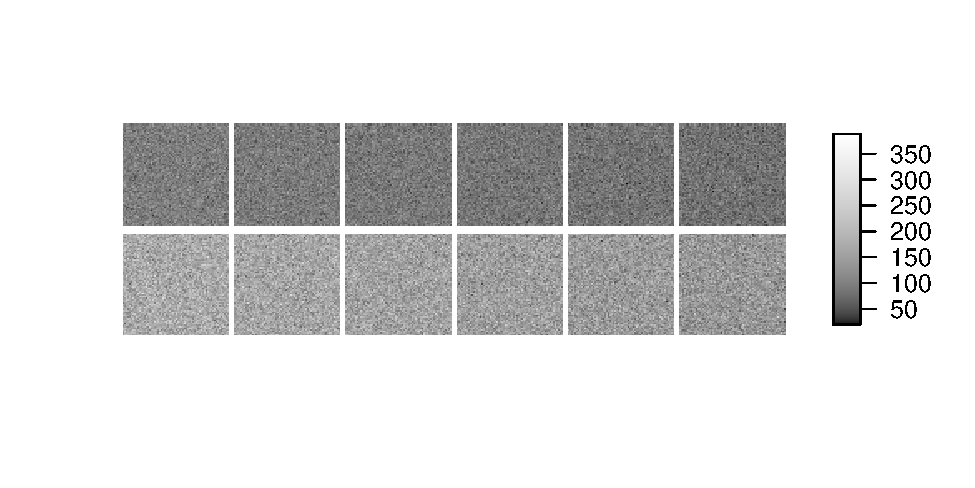
\includegraphics[width=1\linewidth]{phdthesis_files/figure-latex/bleaching-sim-1} \hfill{}

\caption{Frames 1, 100, 200, 300, 400 and 500 from
image series of 100,000 diffusing emitters of brightness
\(\epsilon = 4\) (top) and \(\epsilon = 7\) (bottom) with 15\% (top) and
20\% (bottom) bleaching.}\label{fig:bleaching-sim}
\end{figure}

It may not be obvious that these image series are subject to bleaching
from figure \ref{fig:bleaching-sim}, but we can see it more clearly in
figure \ref{fig:bleaching-sim-mean-intensity}.





\begin{figure}

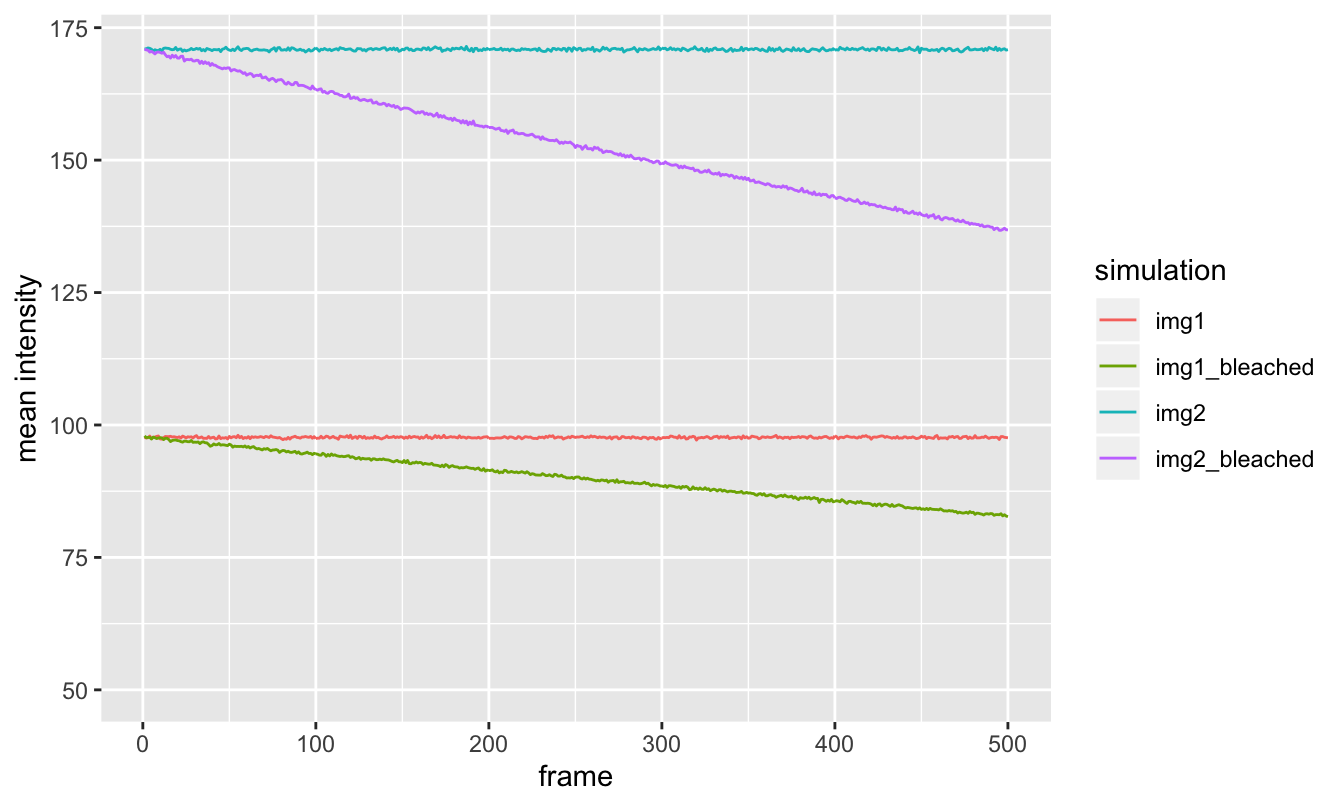
\includegraphics[width=1\linewidth]{phdthesis_files/figure-latex/bleaching-sim-mean-intensity-1} \hfill{}

\caption{Mean intensity profiles of
the simulated image series with and without bleaching. Simulation 1 was
bleached by 15\% and simulation 2 by 20\%.}\label{fig:bleaching-sim-mean-intensity}
\end{figure}

\subsection{FCS}\label{fcs}

The unrelated images \texttt{img1} and \texttt{img2} have a tiny median
cross-correlated brightness of \(B_\text{cc} = 0.0036\), signifying no
significant correlation, as one would expect. However, the bleached
images \texttt{img1\_bleached} and \texttt{img2\_bleached} have a
significant \(B_\text{cc} = 0.3686\). This shows that bleaching is
introducing correlation between otherwise unrelated images. Since
correlation is used as a proxy for hetero-interaction, bleaching can
make it appear as though there is interaction when in fact there is not.

\subsection{FFS}\label{ffs}

\BeginKnitrBlock{definition}[median mean pixel intensity]
\protect\hypertarget{def:unnamed-chunk-31}{}{\label{def:unnamed-chunk-31}
\iffalse (median mean pixel intensity) \fi{} }The \emph{median mean
pixel intensity} of an image series is found by taking the mean
intensity of each pixel in the image series and then taking the median
of those means. It can be thought of as a summary statistic for the
pixel intensity of the image series.
\EndKnitrBlock{definition}

\BeginKnitrBlock{definition}[median pixel intensity variance]
\protect\hypertarget{def:unnamed-chunk-32}{}{\label{def:unnamed-chunk-32}
\iffalse (median pixel intensity variance) \fi{} }The \emph{median pixel
intensity variance} of an image series is found by taking the variance
in the intensity of each pixel in the image series and then taking the
median of those variances. It can be thought of as a summary statistic
for the variance in the pixel intensity of the image series.
\EndKnitrBlock{definition}

In FFS, one is always interested in the mean and variance of pixel
values. \texttt{img1} has a median mean pixel intensity of 98 and a
median pixel intensity variance of 487. The mean brightness is
\(\epsilon = 3.9959\) (very close to 4, as expected since the image
series was simulated with brightness \(\epsilon = 4\)). For
\texttt{img1\_bleached}, we find a median mean pixel intensity of 90 and
a median pixel intensity variance of 468. The mean brightness is
\(\epsilon = 4.2026\). Hence, bleaching has altered both the means and
variances of the pixels, resulting in a change in calculated brightness.
The non-stationary mean frame intensity introduced by bleaching
decreases the mean but increases the variance. The loss in signal has
the effect of slightly decreasing the variance: with Poisson statistics
(such as photon-emission), a loss of signal (photons) leads directly to
a loss in variance. This is a subtle point not discussed anywhere in the
literature; it is shown in figure \ref{fig:visualize-variance-decrease}.







\begin{figure}

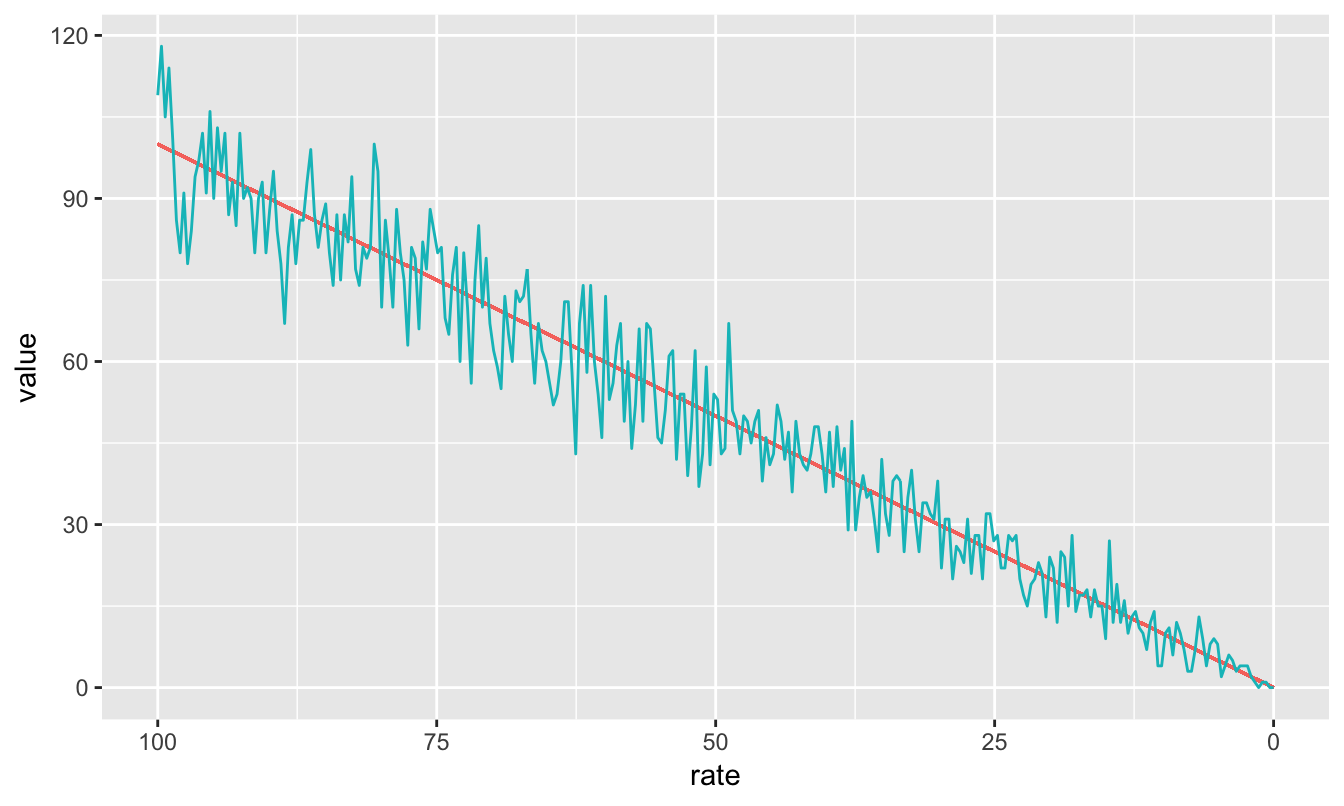
\includegraphics[width=0.9\linewidth]{phdthesis_files/figure-latex/visualize-variance-decrease-1} \hfill{}

\caption{A decrease in the Poisson rate
(e.g.~for emission of photons) leads to a decrease in the mean (blue
line) but also a decrease in fluctuations around the mean. Notice that
towards the right where rate is low, fluctuations around the mean are at
their smallest.}\label{fig:visualize-variance-decrease}
\end{figure}

\section{Exponential fitting
detrending}\label{exponential-fitting-detrending}

Naively, one could assume that bleaching of fluorophores takes place at
some constant rate. This would mean that the intensity of the image
would die-off according to an exponential decay. In figure
\ref{fig:exp-fit-bleach}, we fit an exponential decay to such ideal
data.




\begin{figure}

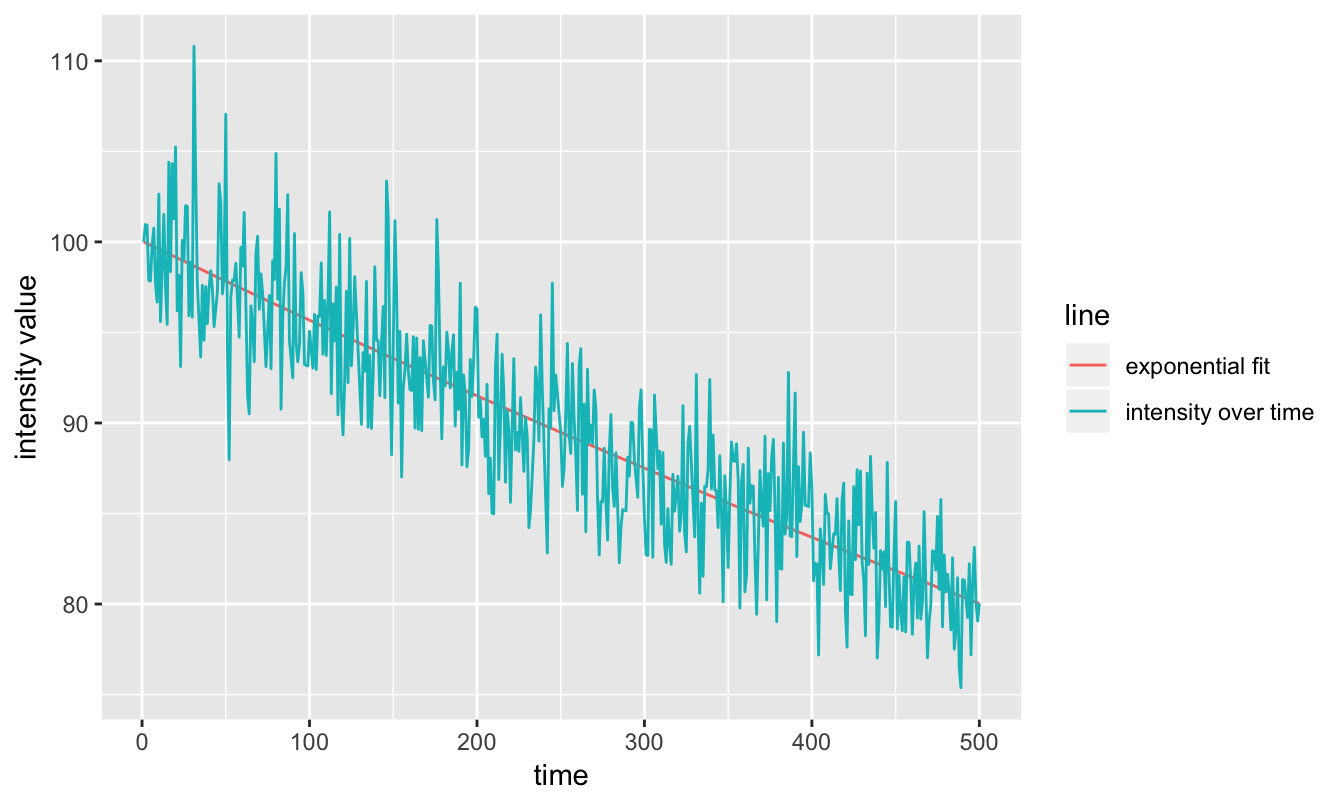
\includegraphics[width=1\linewidth]{phdthesis_files/figure-latex/exp-fit-bleach-1} \hfill{}

\caption{Exponential fit to intensity trace of image
which is subject to bleaching at a constant rate.}\label{fig:exp-fit-bleach}
\end{figure}

Having fit the data, one may record the deviations from the fitted line
as the \emph{fluctuations} and replace these fluctuations about a
straight line, which is placed at the mean of the original series; for
figure \ref{fig:exp-fit-bleach} above, this mean is 90. Figure
\ref{fig:exp-fit-corr} shows the corrected series.








\begin{figure}

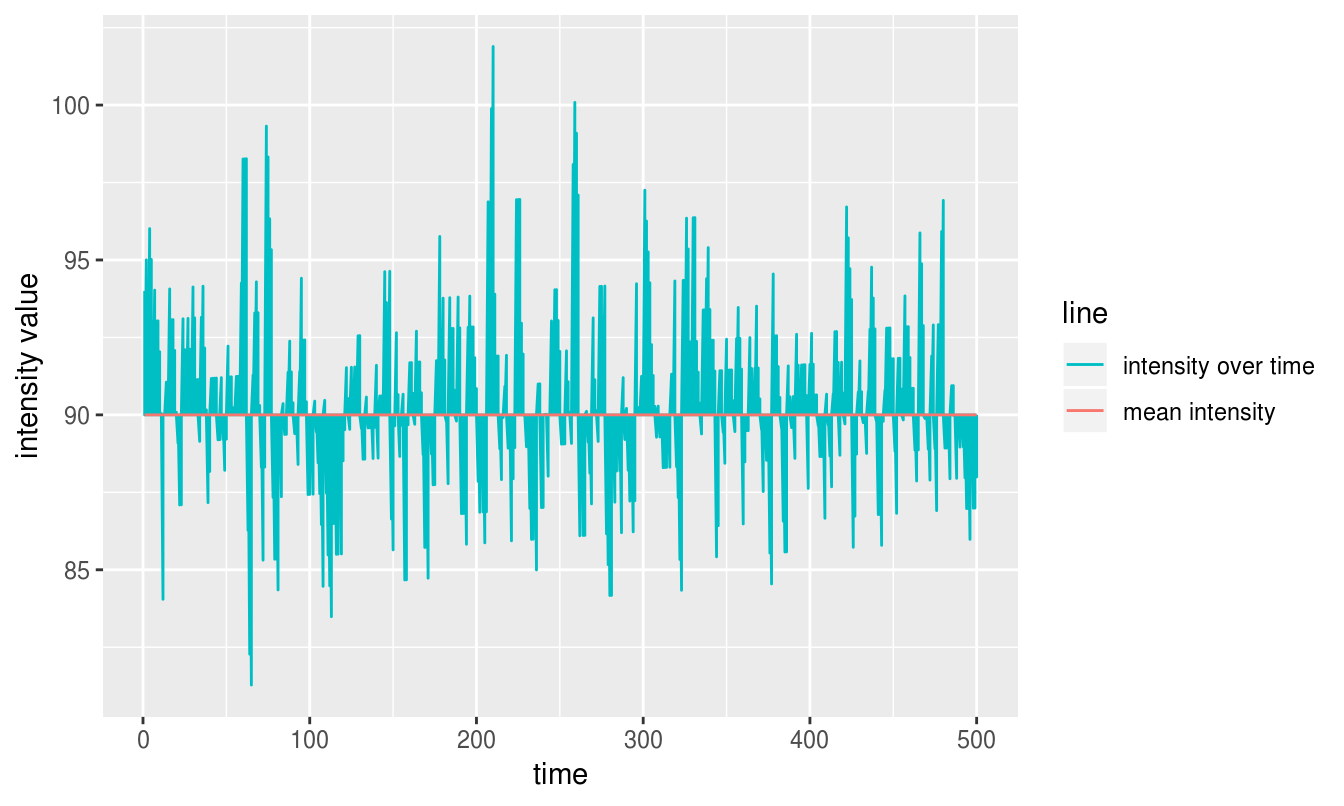
\includegraphics[width=1\linewidth]{phdthesis_files/figure-latex/exp-fit-corr-1} \hfill{}

\caption{The blue line from figure
\ref{fig:exp-fit-bleach} has changed to a straight horizontal line
cutting the \(y\) axis at the mean intensity of the original intensity
trace. The fluctuations about the blue line that existed in figure
\ref{fig:exp-fit-bleach} are preserved here. As an example, see the
large downward fluctuation at \(t \approx 50\) seconds in both figures.}\label{fig:exp-fit-corr}
\end{figure}

We can see that here, in the ideal case where the naive assumptions of
the exponential decay fitting approach hold, this approach works quite
well. Let us now examine the case where these assumptions don't hold
because there are other long-term fluctuations e.g.~due to cell
movement. We add these other fluctuations as a gentle sinusoid. See
figure \ref{fig:exp-decay-with-sin}.




\begin{figure}

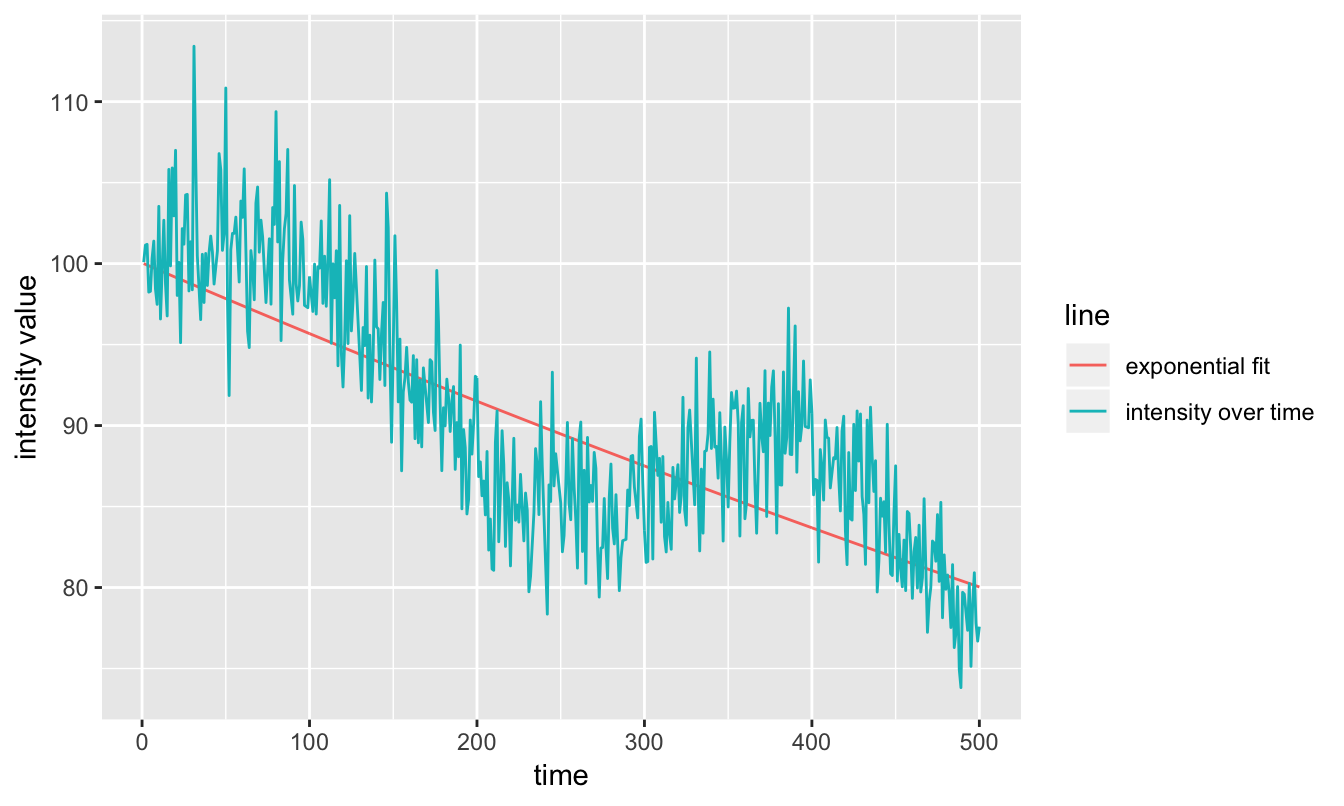
\includegraphics[width=1\linewidth]{phdthesis_files/figure-latex/exp-decay-with-sin-1} \hfill{}

\caption{An exponential decay with added
sinusoidal variance, fit with a simple exponential decay.}\label{fig:exp-decay-with-sin}
\end{figure}

One can see by eye that this is not a good fit for the data. This has
disastrous consequences for the detrended series, shown in figure
\ref{fig:exp-fit-decay-with-sin-corr}.





\begin{figure}

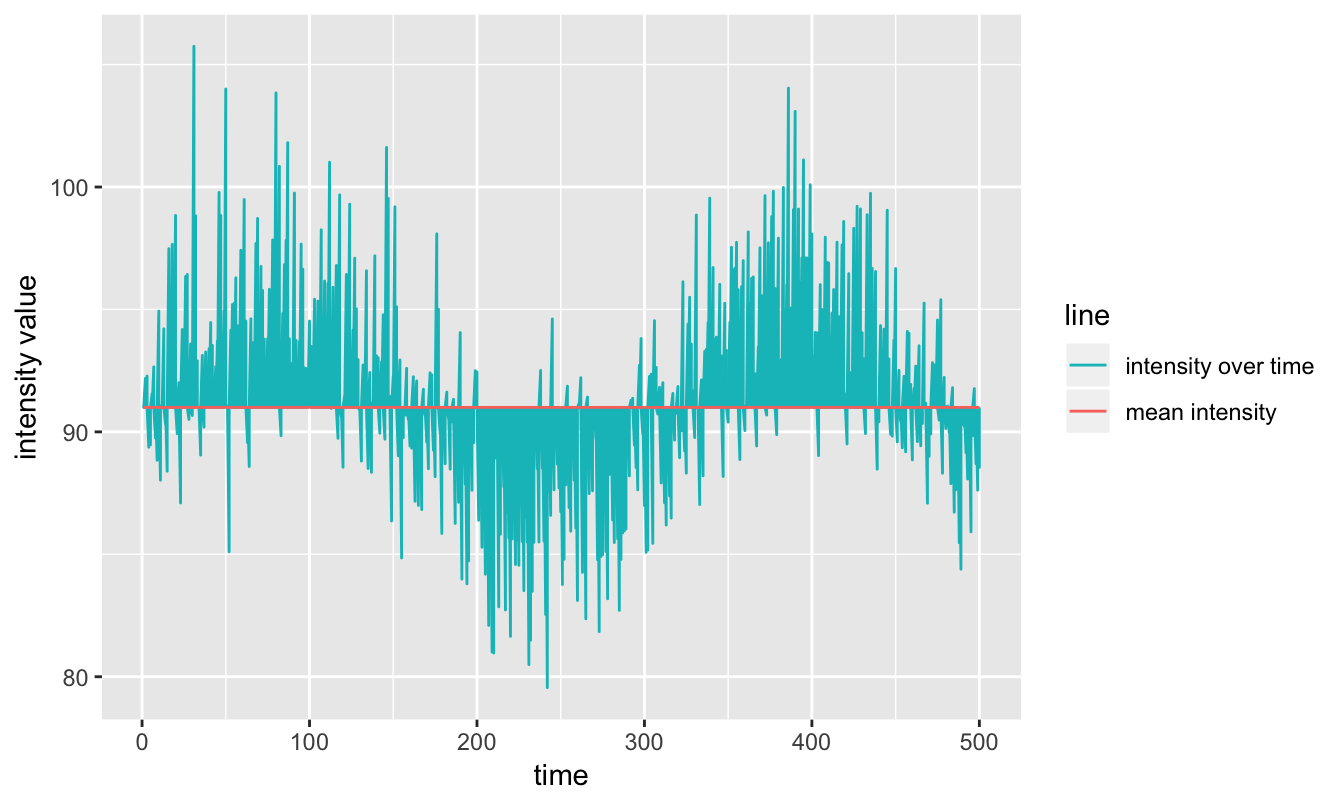
\includegraphics[width=1\linewidth]{phdthesis_files/figure-latex/exp-fit-decay-with-sin-corr-1} \hfill{}

\caption{Result of exponential fitting
detrending applied to a decay with a long-term sinusoidal trend
component.}\label{fig:exp-fit-decay-with-sin-corr}
\end{figure}

One can see in figure \ref{fig:exp-fit-decay-with-sin-corr} that the
exponential fit detrend failed to remove the sinusoidal trend in the
data (even though it \emph{did} remove the exponential decay component).
We have now seen that exponential fitting detrending is appropriate when
the decay has a particular form, but is otherwise not fit for use. This
is a problem common to all fitting approaches to detrending, even the
more flexible types like polynomial detrending \citep{polynomial}. For
this reason alone, for the purpose of detrending, fitting approaches
should be avoided.

\section{Boxcar smoothing detrending}\label{boxcar-smoothing-detrending}

A common approach to obtaining the line from which to measure
deviations/fluctuations (as in the red line in figure
\ref{fig:exp-fit-bleach}) is to \emph{smooth} the time series,
i.e.~construct the line by taking a \emph{local average} at each point.
This is often referred to as \emph{boxcar smoothing} because it can be
visualized as drawing a box around a neighborhood of points, taking
their average as the smoothed value at that point and then moving the
box onto the next series of points and repeating the procedure. See
figure \ref{fig:boxcar-explanation}.










\begin{figure}

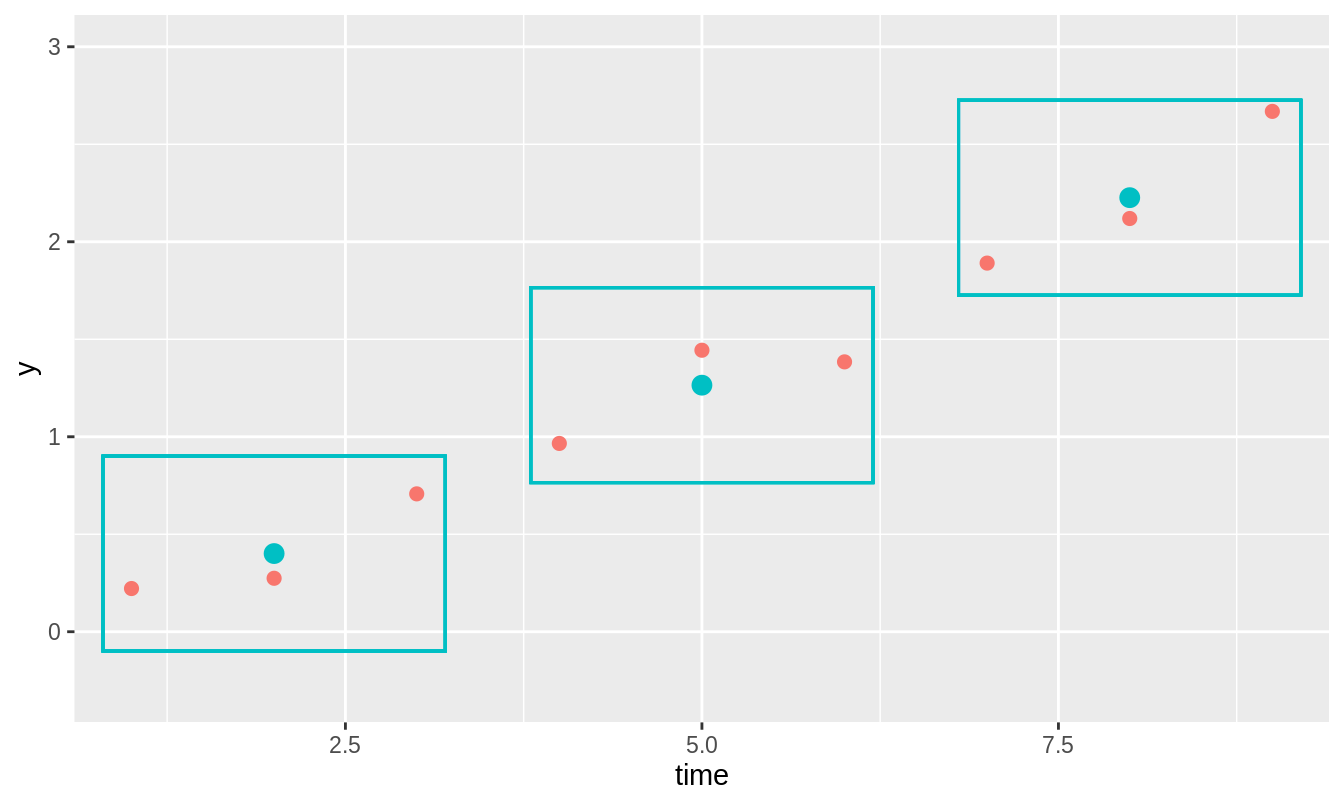
\includegraphics[width=1\linewidth]{phdthesis_files/figure-latex/boxcar-explanation-1} \hfill{}

\caption{The original time series is depicted by
the red dots. The blue rectangles represent the \emph{boxcar}. This
boxcar is said to be of length 3 because it is wide enough to encompass
3 points at a time. The boxcar is centered on a point and then the
smoothed value at that point (blue dot) is calculated as the mean value
of all points within the boxcar. In reality, every point gets a smoothed
value which means that the boxcar \emph{overlaps} but in this figure,
for the sake of clarity, they are not overlapped.}\label{fig:boxcar-explanation}
\end{figure}

The parameter \(l\) of a boxcar is such that the length of the boxcar is
equal to \(2l + 1\). This ensures that the length of the boxcar is
always odd) which means it can always be centered upon a point). Hence
the allowable lengths of a boxcar are \(3,5,7,9,\) etc.

The boxcar parameter \(l\) has a large effect on the type of smoothing
achieved. This can be seen in figure \ref{fig:boxcar-sizes} where boxcar
smoothing is applied to the trace in figure \ref{fig:exp-fit-bleach}.
The traces for \(l=1\) and \(l=3\) are far too wiggly (not smooth
enough); the trace for \(l=75\) is better but perhaps still slightly
wiggly; finally, the traces for \(l=300\) and \(l=1000\) are too close
to straight horizontal lines (too smooth).





\begin{figure}

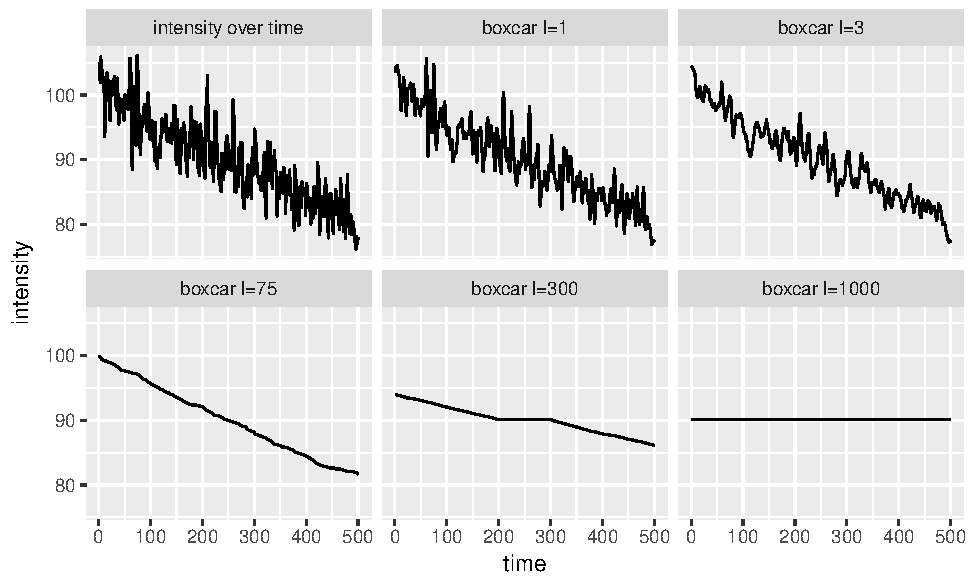
\includegraphics[width=1\linewidth]{phdthesis_files/figure-latex/boxcar-sizes-1} \hfill{}

\caption{The original intensity trace is shown in the
top-left. The other panels show the result of boxcar smoothing for
\(l = 1, 3, 75, 300\) and \(1000\).}\label{fig:boxcar-sizes}
\end{figure}

This begs the question: what is the correct smoothing parameter \(l\)?

\section{Choosing the correct smoothing parameter for
detrending}\label{choosing-the-correct-smoothing-parameter-for-detrending}

Figure \ref{fig:boxcar-sizes} shows that the choice of boxcar size is
crucial because different sizes lead to very different ``smoothed''
lines. The most common choice in the community is to choose \(l = 10\)
\citep{SimFCS}. There is no justification for this choice.

In section \ref{number-and-brightness}, we learned that for immobile
particles, the expected brightness is \(B = 1\). This fact can be used
to solve for the appropriate choice of \(l\) to use for detrending a
specific image series.

\BeginKnitrBlock{definition}
\protect\hypertarget{def:unnamed-chunk-33}{}{\label{def:unnamed-chunk-33}
}The \emph{mean intensity profile} of one channel of an image series is
obtained by calculating the mean intensity of each frame in that image
series.
\EndKnitrBlock{definition}

The mean intensity profile can be used to visualize the bleaching of an
image series. If the fluorophores are bleaching, the mean intensity
should be decreasing over time. To proceed with solving for the
appropriate \(l\), we need to make one assumption. This is that any two
image series with the same mean intensity profile are appropriately
detrended with the same detrending parameter \(l\). This assumption
seems reasonable to me, however there is no need to debate its validity
because later, detrending with the solved-for parameter \(l\) will be
evaluated with simulated data and compared to the standard \(l = 10\).
If this assumption is bad, then the performance of the detrending that
relies on it should also be bad. With this assumption in hand, solving
for \(l\) proceeds as follows:

\begin{enumerate}
\def\labelenumi{\arabic{enumi}.}
\tightlist
\item
  Simulate an image series with immobile particles only which has the
  same mean intensity profile as the acquired real data.
\item
  Given that the simulated series is of immobile particles only, once
  properly detrended, it should have \(B = 1\).
\item
  The \(l\) for which the detrended series has mean brightness closes to
  1 is the most appropriate for the simulated data.
\item
  By the assumption above, this \(l\) is the most appropriate for the
  real data.
\end{enumerate}

Mathematically, this can be expressed as

\begin{equation}
l = \text{argmin}_{\tilde{l}} (1 - |\text{ mean brightness of simulated series detrended with parameter } \tilde{l}|)
\label{eq:leq}
\end{equation}

In fact, what I have done here is to give a general method for solving
for any detrending parameter \(\alpha\):

\begin{equation}
\alpha = \text{argmin}_{\tilde{\alpha}} (1 - |\text{ mean brightness of simulated series detrended with parameter } \tilde{\alpha}|)
\label{eq:detrend-param}
\end{equation}

This will be useful later when other detrending regimes with their own
parameters are introduced.

\section{Exponential smoothing
detrending}\label{exponential-smoothing-detrending}

\emph{Exponential smoothing} is a slight alteration to boxcar smoothing.
The idea is that when computing a local average, points nearer to the
point of interest should have greater weights.\footnote{\url{https://en.wikipedia.org/wiki/Weighted_arithmetic_mean}}
The weights fall off with distance \(|t|\) from the point of interest
according to \(\exp(-\frac{|t|}{\tau})\) where the parameter \(\tau\) is
a positive real number. This function is visualized in figure
\ref{fig:exp-smooth-func}. For small values of \(\tau\), only values
very close to the point of interest have importance when calculating the
local average. For larger values of \(\tau\), further values also have
importance (but closer values always have higher weights). In this
sense, increasing the value of \(\tau\) has a similar effect to
increasing the value of \(l\) for the boxcar in that further away points
are taken into account.






\begin{figure}

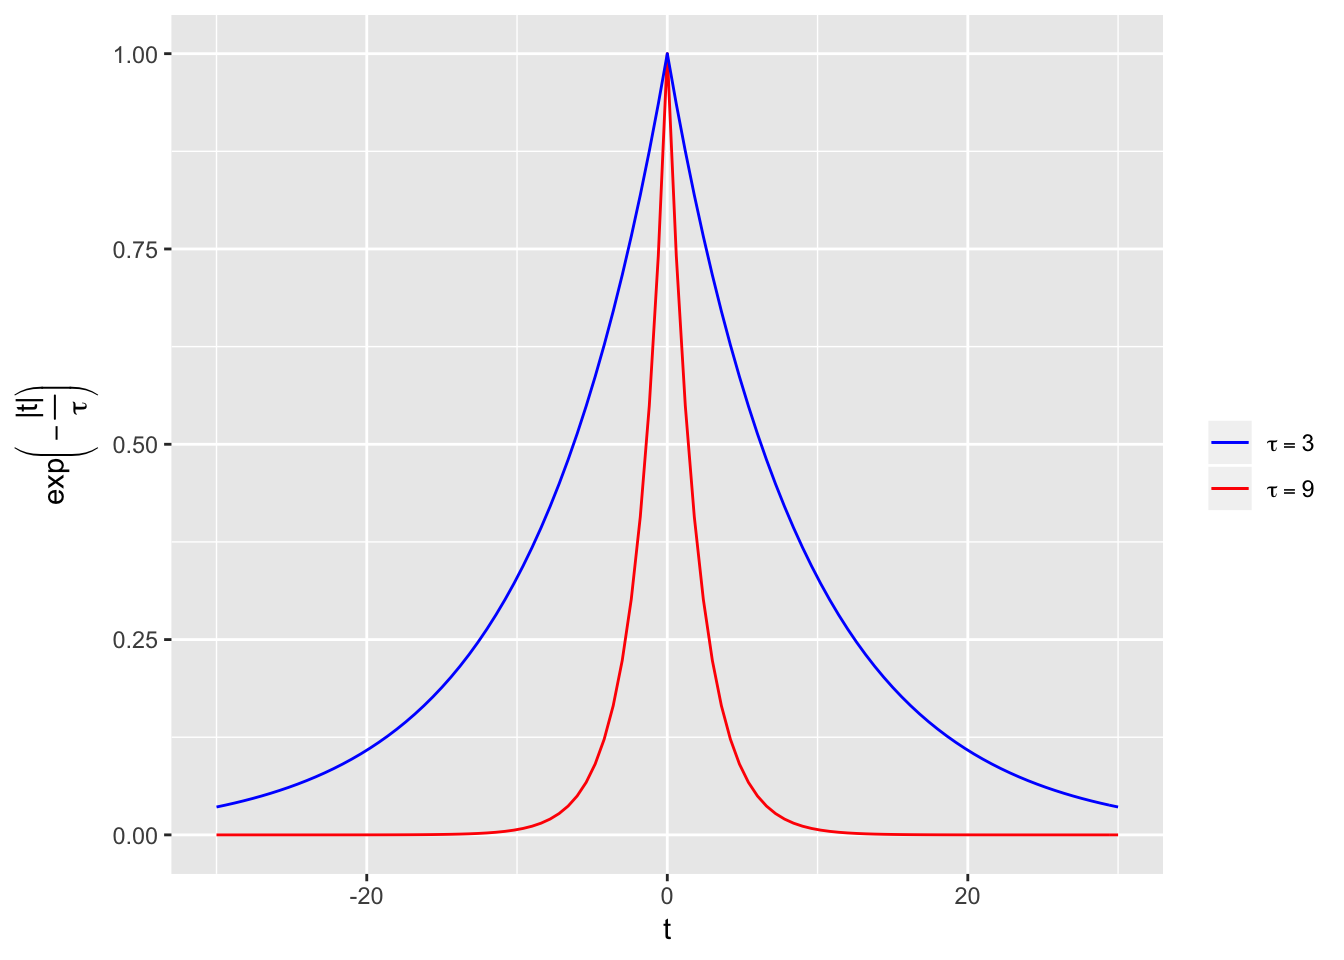
\includegraphics[width=1\linewidth]{phdthesis_files/figure-latex/exp-smooth-func-1} \hfill{}

\caption{The function \(\exp(-\frac{|t|}{\tau})\)
visualized with \(\tau = 3\) and \(\tau = 9\). For \(\tau = 3\), points
at distance \(|t| = 10\) have approximately zero weight, whereas for
\(\tau = 9\), these points have significant weight.}\label{fig:exp-smooth-func}
\end{figure}

In figure \ref{fig:tau-values}, exponential smoothing with different
parameters \(\tau\) is applied to the trace in figure
\ref{fig:exp-fit-bleach}. The results are similar to those in figure
\ref{fig:boxcar-sizes}.





\begin{figure}

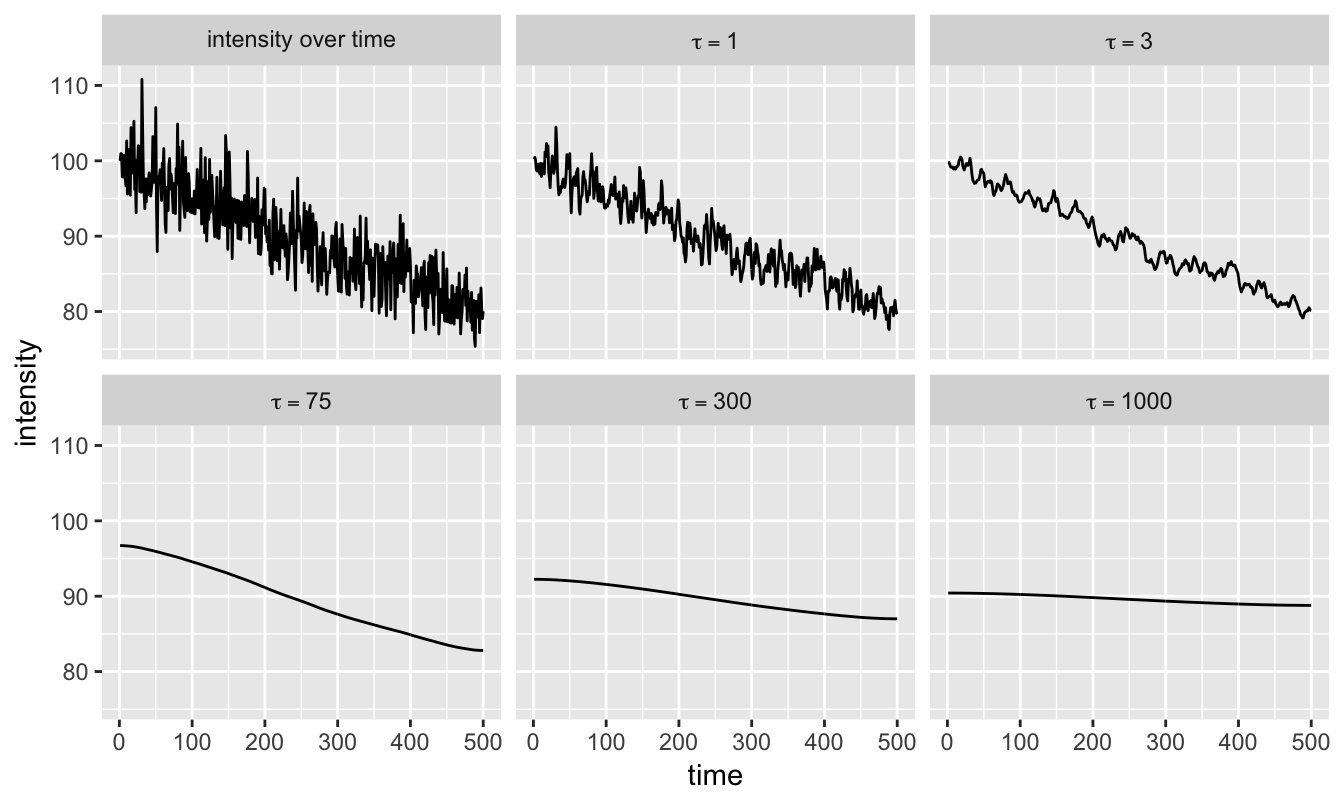
\includegraphics[width=1\linewidth]{phdthesis_files/figure-latex/tau-values-1} \hfill{}

\caption{The original intensity trace is shown in the
top-left. The other panels show the result of exponential smoothing for
\(\tau = 1, 3, 75, 300\) and \(1000\).}\label{fig:tau-values}
\end{figure}

Heuristically, exponential smoothing detrending seems favorable to
boxcar detrending because the idea that points further away from the
point of interest are less important (but still somewhat important) when
computing the local average is reasonable. Indeed, this was the method
proposed in the original number and brightness paper \citep{NB}. For
this reason, exponential smoothing was the method of choice for my paper
where the method of choosing the correct detrending parameter was
published \citep{nandb}.

\section{Correcting for non-stationary
variance}\label{correcting-for-non-stationary-variance}

\BeginKnitrBlock{definition}
\protect\hypertarget{def:unnamed-chunk-34}{}{\label{def:unnamed-chunk-34}
}The variance of a random variable \(X\) is the expected value of the
squared deviation of \(X\) from its mean \(\mu\):

\begin{equation}
\text{Var}(X) = E[(X - \mu)^2]
\label{eq:variance}
\end{equation}
\EndKnitrBlock{definition}

All of this chapter so far has focused on correcting for non-stationary
mean. As shown in figure \ref{fig:visualize-variance-decrease}, as the
mean decreases, so too does the variance. For an instance \(x\) of the
random variable \(X\) with expected value \(E[X] = \mu\), \(x - \mu\) is
the \emph{deviation} of \(x\) from \(\mu\). If we write \(x\) as
\(x = \mu + \tilde{x}\), then we get the deviation
\(x - \mu = (\mu + \tilde{x}) - \mu = \tilde{x}\), so \(\tilde{x}\) is
the deviation. For a given point in figure
\ref{fig:visualize-variance-decrease}, its deviation is its distance
from the red line. For positive real number \(k\), making the
transformation \(\tilde{x} \rightarrow \sqrt{k}\tilde{x}\) i.e.
\(x \rightarrow \mu + \sqrt{k}\tilde{x}\) causes the variance (i.e.~the
\emph{squared deviation}) to be transformed as
\(\text{Var}(X) \rightarrow k \times \text{Var}(X)\). Hence, we have a
way to modify the variance of a time series as a whole by modifying the
deviation of each time point from the mean. For months, I toyed with
this idea as a solution of correcting for non-stationary variance.
However, in reality the contribution to the variance in intensity at a
given pixel is down to both Poisson photon statistics and fluorophore
movement. This combination of factors makes it very difficult to
ascertain the amount by which the variance should be altered. I
eventually abandoned my efforts to alter the variance like this in favor
of the \emph{Robin Hood} detrending algorithm (section
\ref{robin-hood-detrending}) which includes correction for
non-stationary variance as an intrinsic part of its detrending routine.

\section{Caveats of fitting and smoothing approaches to
detrending}\label{caveats-of-fitting-and-smoothing-approaches-to-detrending}

Both fitting and smoothing approaches to detrending have serious
caveats. Fitting approaches assume that the fluorescence intensity decay
has a certain form. Unpredictable issues such as cell movement mean that
no particular decay form can be assumed. Smoothing methods do not
perform well at the edges of time series that they are applied to. They
also require the user to choose a smoothing parameter. The problem of
how to best choose this parameter was solved recently \citep{nandb}, but
this method has not been widely adopted. Most importantly, both fitting
and smoothing fail when the data cannot be approximated as continuous
(fitted and smoothed lines are continuous approximations of data).
Fluorescence intensity data at low intensities---where most pixel values
are either 0 or 1---are quasi-binary\footnote{By \emph{quasi-binary}, I
  just mean that almost all values are 0 or 1.} and hence a continuous
approximation does not make sense (see figure
\ref{fig:fit-smooth-caveats}). This means that neither fitting nor
smoothing are applicable detrending methods at low intensities. This is
the crucial caveat of these methods because, when bleaching is a
problem, it is common to reduce laser power to reduce bleaching, which
leads directly to lower intensity images. With fitting and smoothing
techniques, it may sometimes be advisable to increase the laser power to
achieve higher intensities such that the detrending routines will
function properly. This means one may need to bleach more in order to be
able to correct for bleaching. This farcical situation necessitates a
new detrending technique which can function at low intensities.







\begin{figure}

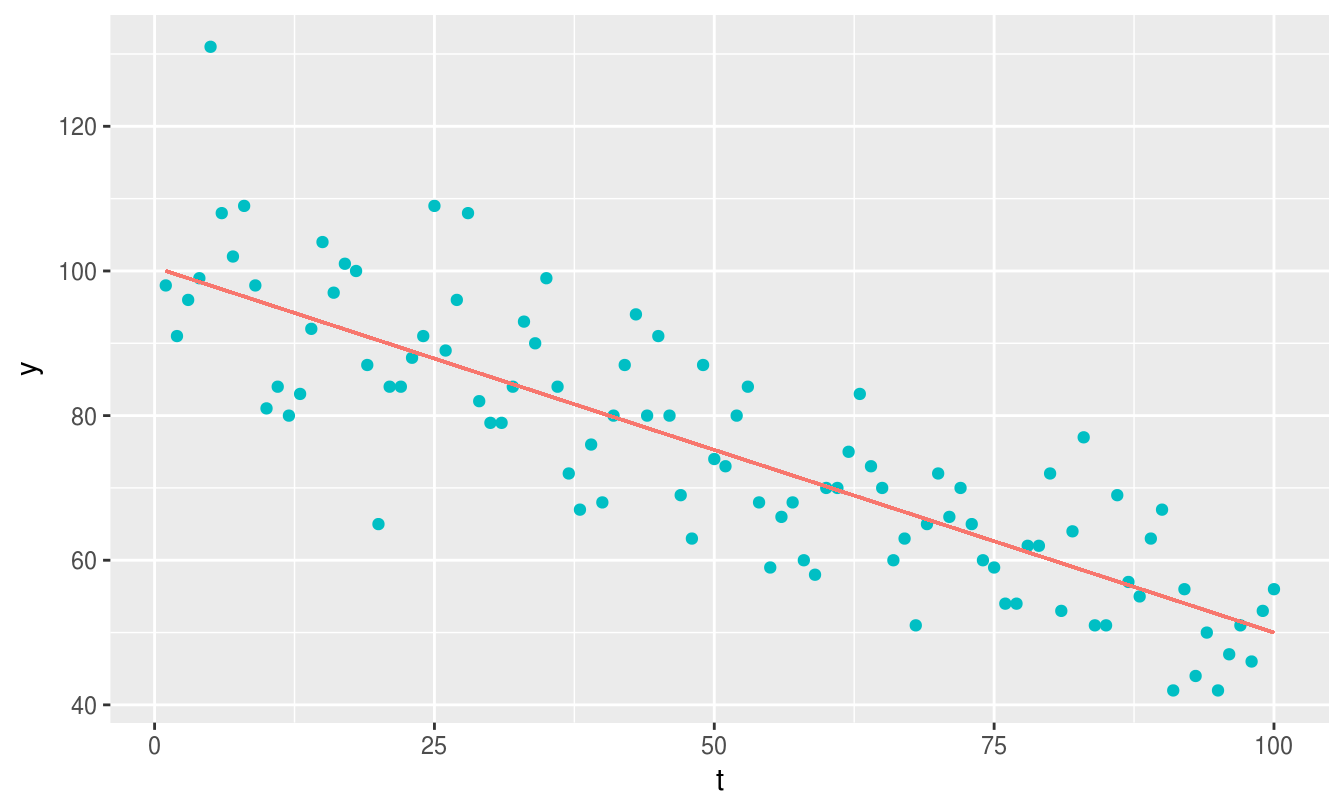
\includegraphics[width=0.49\linewidth]{phdthesis_files/figure-latex/fit-smooth-caveats-1} 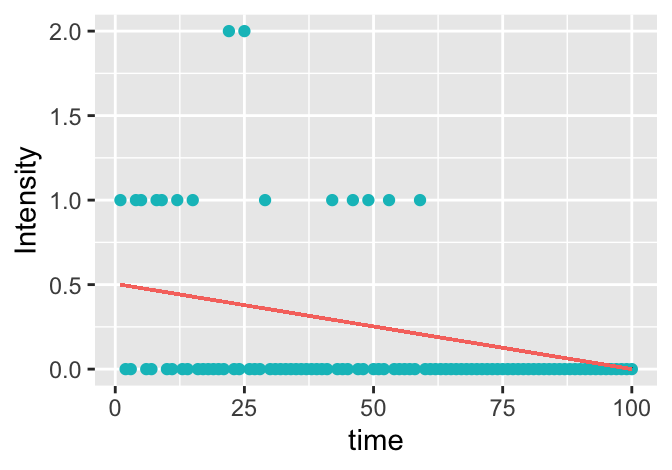
\includegraphics[width=0.49\linewidth]{phdthesis_files/figure-latex/fit-smooth-caveats-2} \hfill{}

\caption{Left: for high (\(\gg 1\)) intensity
values, the line is a satisfactory approximation of the data,
representing it well. Right: for low (quasi-binary) intensity values,
the line is not a good approximation for the data and indeed no line or
curve could represent the data well.}\label{fig:fit-smooth-caveats}
\end{figure}

\section{Robin Hood detrending}\label{robin-hood-detrending}

Intensity images in units of photons are count data. This means that the
values are all natural numbers, i.e.~elements of
\(\mathbb{N}_0=\{0, 1, 2, 3, \ldots\}\). Fitting and smoothing give
real-numbered values (elements of \(\mathbb{R}\)), which must then be
transformed back into count data (elements of \(\mathbb{N}_0\)),
normally by rounding. This means that fitting and smoothing methods of
detrending push values through
\(\mathbb{N}_0 \rightarrow \mathbb{R} \rightarrow \mathbb{N}_0\). When
current methods were failing to properly detrend low-intensity images, I
began to wonder was it necessary to go through the real numbers
\(\mathbb{R}\), given that the start and end points were the natural
numbers \(\mathbb{N}_0\)?

Consider figure \ref{fig:rh-detrend-eg}. There is a bleached and
unbleached version of an intensity trace. Suppose that our real data is
the bleached trace, but we \emph{wish} it looked like the unbleached
trace. You may wonder why the unbleached trace is not at the starting
intensity of the bleached series. For reasons that will become clear,
the Robin Hood algorithm can only place the detrended image at the mean
intensity of the original image. This is not a problem because the issue
with bleaching in FCS and FFS is mainly that the changing signal leads
to incorrect calculations, not that the loss in signal leads to a
chronic lack of information (photons). Indeed a feature of the Robin
Hood algorithm is that it preserves the mean intensity of the real data
on a pixel-by pixel basis.



\begin{figure}

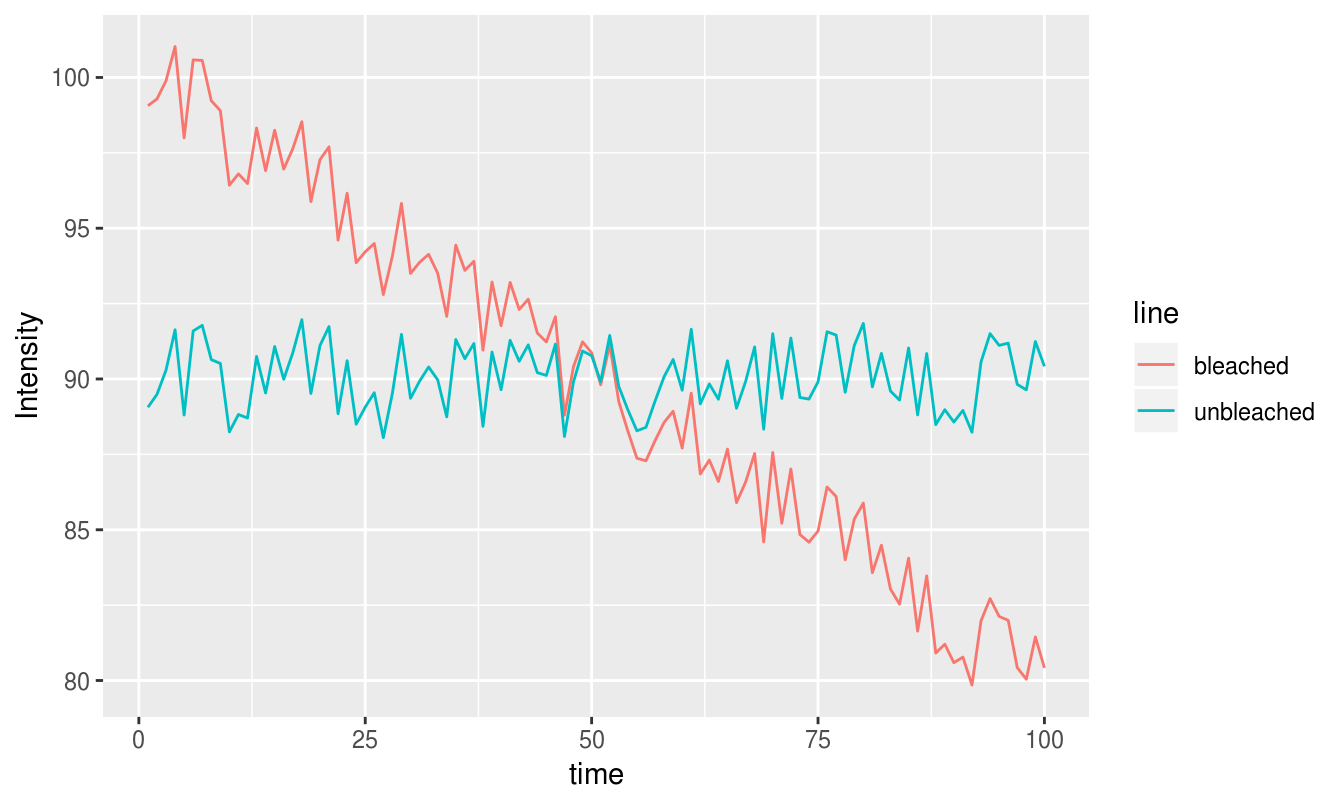
\includegraphics[width=1\linewidth]{phdthesis_files/figure-latex/rh-detrend-eg-1} \hfill{}

\caption{Bleached and unbleached intensity traces.}\label{fig:rh-detrend-eg}
\end{figure}

To get to the unbleached intensity trace from the bleached intensity
trace, intensity must be subtracted from time-points with too much
intensity and added to time points with too little intensity. This can
be done by \emph{taking} counts from frames with too much intensity and
\emph{giving} them to frames with too little intensity. In this way, no
counts are gained or lost, they are just moved around the image series.
See figure \ref{fig:rh-lego}. Counts are passed from one frame to
another \emph{along} a given pixel, i.e.~if a count is taken from pixel
at position \(p\) in some frame \(i\), it must be given to a pixel at
the same position \(p\) in some other frame \(j\). It is this condition
that ensures that the mean intensity images of the original and
detrended image series are the same.






\begin{figure}

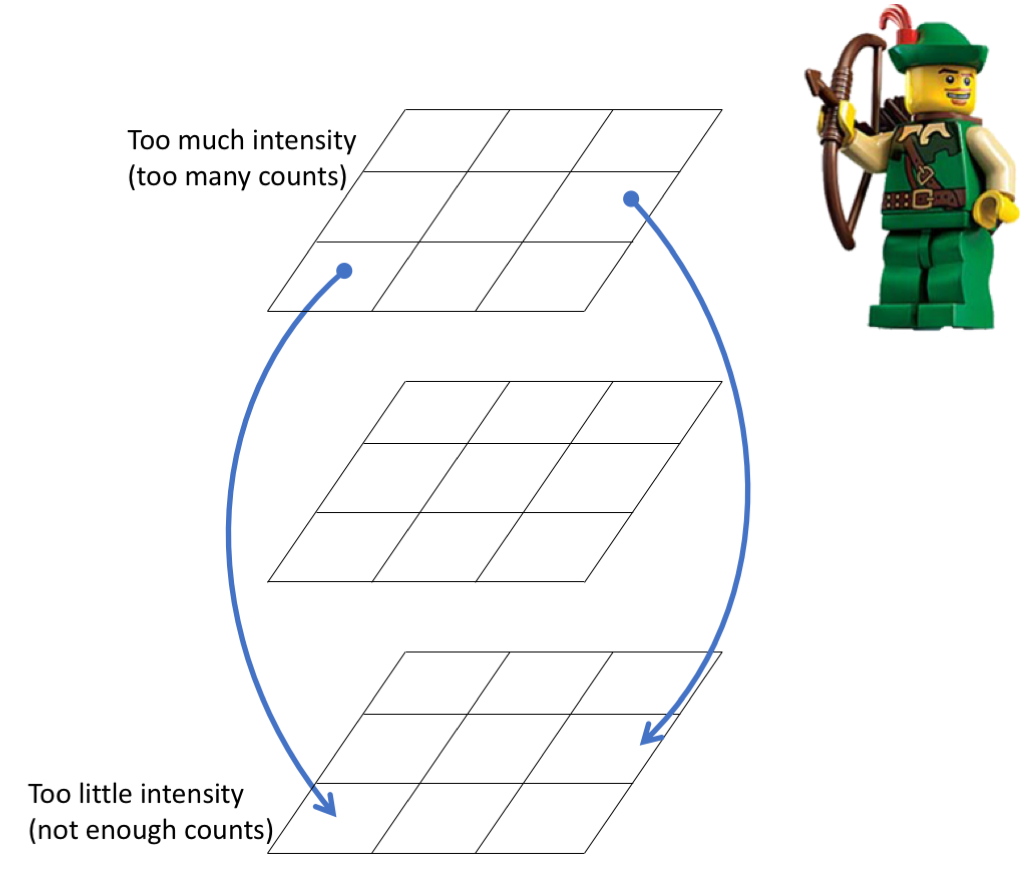
\includegraphics[width=0.48\linewidth]{/home/travis/build/rorynolan/phdthesis/img/rh} 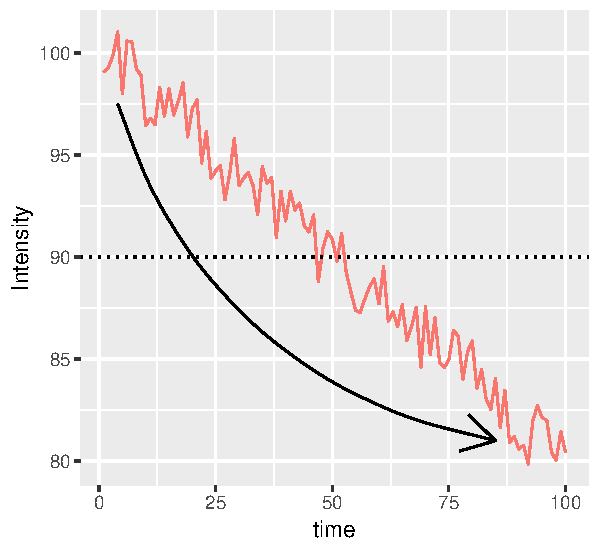
\includegraphics[width=0.48\linewidth]{/home/travis/build/rorynolan/phdthesis/img/rh_lego_plot} \hfill{}

\caption{Robin Hood: counts are taken from frames of higher
intensity (usually closer to the start of the image series) and given to
frames of lower intensity (usually closer to the end of the image
series).}\label{fig:rh-lego}
\end{figure}

To determine how many swaps need to be made to detrend a given image
series, equation \eqref{eq:detrend-param} can be used, with \(\alpha\)
being the number of swaps.

The random gifting of counts from higher to lower intensity frames has
the effect of redistribution mean intensity but \emph{also} variance in
intensity. With photon statistics (which follow a Poisson distribution),
random counts provide both mean and variance. This is in contrast to all
previous methods which consist of determining local deviation and adding
it to a \emph{fixed} global mean: this provides no redistribution of
variance.

\section{A comparison of detrending methods}\label{detrend-compare}

To compare the various detrending methods, I use the following workflow:

\begin{enumerate}
\def\labelenumi{\arabic{enumi}.}
\tightlist
\item
  Simulate a number \(N = 100,000\) of particles diffusing with known
  diffusion rate. Simulations were done with the \texttt{brownded}
  software package (section \ref{brownded}).
\item
  Simulate photon emission from these particles with chosen brightness
  \(\epsilon\) and create an image series from this, being careful to
  (virtually) sample at a rate appropriate for number and brightness
  analysis.
\item
  Bleach the simulation with a chosen constant bleaching rate.
\item
  Simulate photon emission from the bleached simulation (bleached
  particles don't emit photons) with the same brightness \(\epsilon\)
  and create an image series.
\item
  Detrend the bleached image series.
\item
  Evaluate the detrending algorithm by measuring how close the
  brightness of the detrended bleached image series is to the known
  simulated brightness.
\end{enumerate}

For all combinations of brightnesses of
\(\epsilon = 0.001, 0.01, 0.1, 1, 10\) and bleaching fractions of 0\%,
1\%, 5\%, 10\%, 15\%, 20\%, 25\%, 30\%, 20 images of 64x64 pixels and
5,000 frames were simulated using 100,000 fluorescent diffusing
particles.\footnote{The simulation took 3 weeks.} These were detrended
with the following detrending routines:\footnote{The detrending took 2
  weeks.}

\begin{enumerate}
\def\labelenumi{\arabic{enumi}.}
\tightlist
\item
  Boxcar with \(l = 10\) (\texttt{boxcar10}, the most common detrending
  routine).
\item
  Exponential smoothing with automatically chosen parameter \(\tau\)
  (\texttt{autotau}).
\item
  Robin Hood with automatically chosen swaps (\texttt{robinhood}).
\end{enumerate}

The performance was evaluated using the \emph{mean relative error}.

\BeginKnitrBlock{definition}
\protect\hypertarget{def:unnamed-chunk-35}{}{\label{def:unnamed-chunk-35} }
For a given brightness and bleaching fraction,

\begin{equation}
\text{mean relative error } = \frac{|(\text{calculated brightness after detrending}) - (\text{true brightness})|}{(\text{true brightness})}
\label{eq:mean-relative-error}
\end{equation}
\EndKnitrBlock{definition}

Figure \ref{fig:detrend-compare} shows the results. Before I discuss
them, note that the common brightnesses that we see are in the range
\(\epsilon = 0.003\) to \(\epsilon = 0.1\).






\begin{figure}

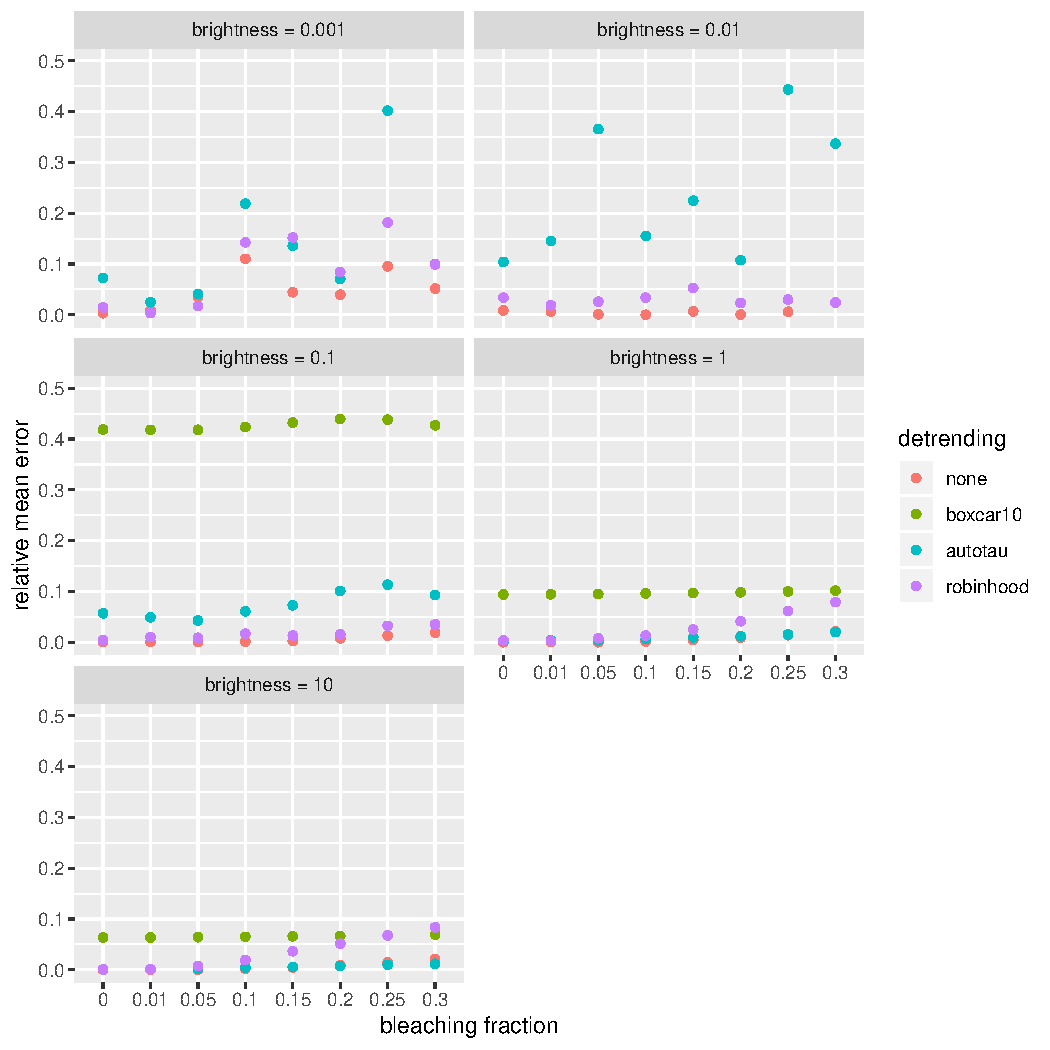
\includegraphics[width=1\linewidth]{/home/travis/build/rorynolan/phdthesis/img/detrend_compare} \hfill{}

\caption{A comparison of different detrending
methods with various brightnesses and bleaching fractions (steady,
constant-rate bleaching), including the results of not detrending at
all.}\label{fig:detrend-compare}
\end{figure}

The most striking thing about figure \ref{fig:detrend-compare} is that
the best choice in all cases is to not detrend at all! This is an
interesting result and seems to render all detrending routines
worthless. However, when working with real data, not detrending does not
work well at all. This will be shown in chapter \ref{applications}. This
is probably because with real data, bleaching is likely not taking place
at a constant, steady rate and other factors such as cell movement are
contributing to medium and long term intensity fluctuations and these
have a detrimental effect on calculations if not detrended out. It would
be possible to study this by mimicking real bleaching profiles with
simulations (see section \ref{mimic}.

The worst performer by far is \texttt{boxcar10}. For example, at
\(\epsilon = 0.1\), it makes an error of worse than 40\% and for
\(\epsilon = 0.001, 0.01\), its error is worse than 50\%, so it does not
even appear on the plot. This is good evidence that arbitrarily choosing
the parameter \(l\) very bad practice. For realistic brightnesses
(\(\le 0.1\)), \texttt{robinhood} is the best with errors almost always
lower than 5\%. \texttt{autotau} also performs very well, with errors
almost always less than 10\%. At the lowest brightness
\(\epsilon = 0.001\), all methods are somewhat erratic. That is because
at this extremely low brightness, there is a critical lack of
information (photons) for the algorithms to work with. Finally, at
unrealistically high brightnesses of \(\epsilon = 1, 10\),
\texttt{autotau} begins to perform well because at these high photon
counts, the caveats of smoothing have totally disappeared. However, I
cannot explain the degradation in the performance of \texttt{robinhood}
in this case. Fortunately, there is no need to dwell on this, as this
situation (\(\epsilon = 1, 10\)) does not arise in practice because
available fluorophores are not this bright.

\chapter{Applications}\label{applications}

\section{Dimerization of FKBP12}\label{dimerization-of-fkbp12}

\subsection{Introduction}\label{introduction}

Myristoylated FKBP12 is known to dimerize upon addition of the drug
AP1510 \citep{Amara}. As a test application of exponential smoothing
detrending (section \ref{exponential-smoothing-detrending}) with
automatically chosen parameter \(\tau\), we used this system with number
and brightness to verify this dimerization. We tested this in 20 Cos7
cells with mClover-labelled FKBP12.

\subsection{Experimental results and
discussion}\label{experimental-results-and-discussion}

We found a brightness increase in \(\epsilon\) of \(\approx 1.6\)-fold
using the \emph{automatic} detrending method. The choice of \(\tau=10\)
resulted in a \(\approx 0.7\)-fold calculated increase, which is indeed
a decrease. The \(\approx 1.6\)-fold increase suggests that dimerization
had occurred (see figure \ref{fig:FKBPfoldchanges}), however, we
expected the increase to be \(\approx 2\)-fold upon dimerization. In
that publication \citep{nandb}, we postulated that the 1.6 figure was
due to the fact that not all of the protein had dimerized. Recently, a
paper came out \citep{fpcompare} explaining how the assumption that all
fluorophores emit signal is invalid and that because of this, oligomeric
state changes calculated from brightness must be adjusted by a
correction factor specific to the fluorophore. Unfortunately, this study
did not characterize mClover, so we do not know its correction factor. I
suspect that applying this correction would bring our figure of 1.6 a
lot closer to 2. We also tried \(\tau=10\), which gave a decrease in
brightness, showing that arbitrary parameter choices lead to
unpredictable and unreliable results and should hence be avoided.





\begin{figure}

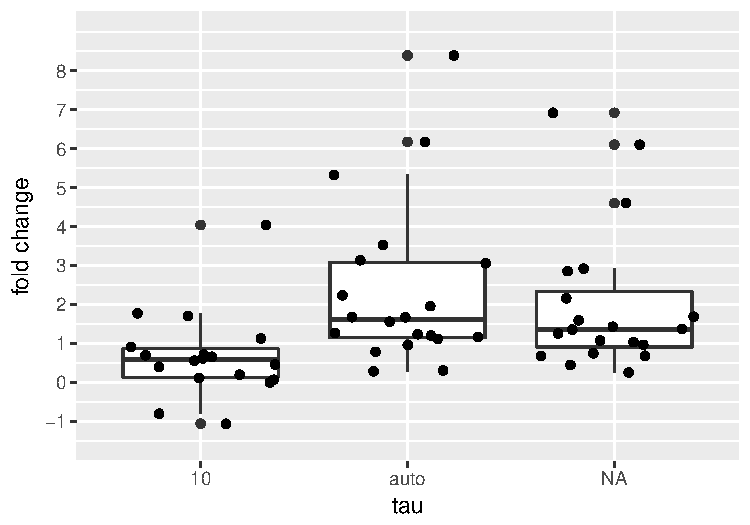
\includegraphics[width=1\linewidth]{/home/travis/build/rorynolan/phdthesis/img/foldchanges} \hfill{}

\caption{The fold changes in brightness
\(\epsilon\) upon addition of AP1510 drug shown for different detrending
routines. \(\tau=\) NA is no detrend.}\label{fig:FKBPfoldchanges}
\end{figure}

The heterogeneity of fold-changes in \(\epsilon\) measured from single
images as shown in figure \ref{fig:FKBPfoldchanges} shows that many
replicates are needed in number and brightness experiments in order to
converge upon the true value of the fold change.

A pair of cells from this study together with their brightness
statistics are shown in figure \ref{fig:nandb-fig}. Notice how there is
no discernible change in intensity before and after addition of the
drug, but there is a discernible change in brightness \(B\), best seen
using the histogram of pixel brightnesses.










\begin{figure}

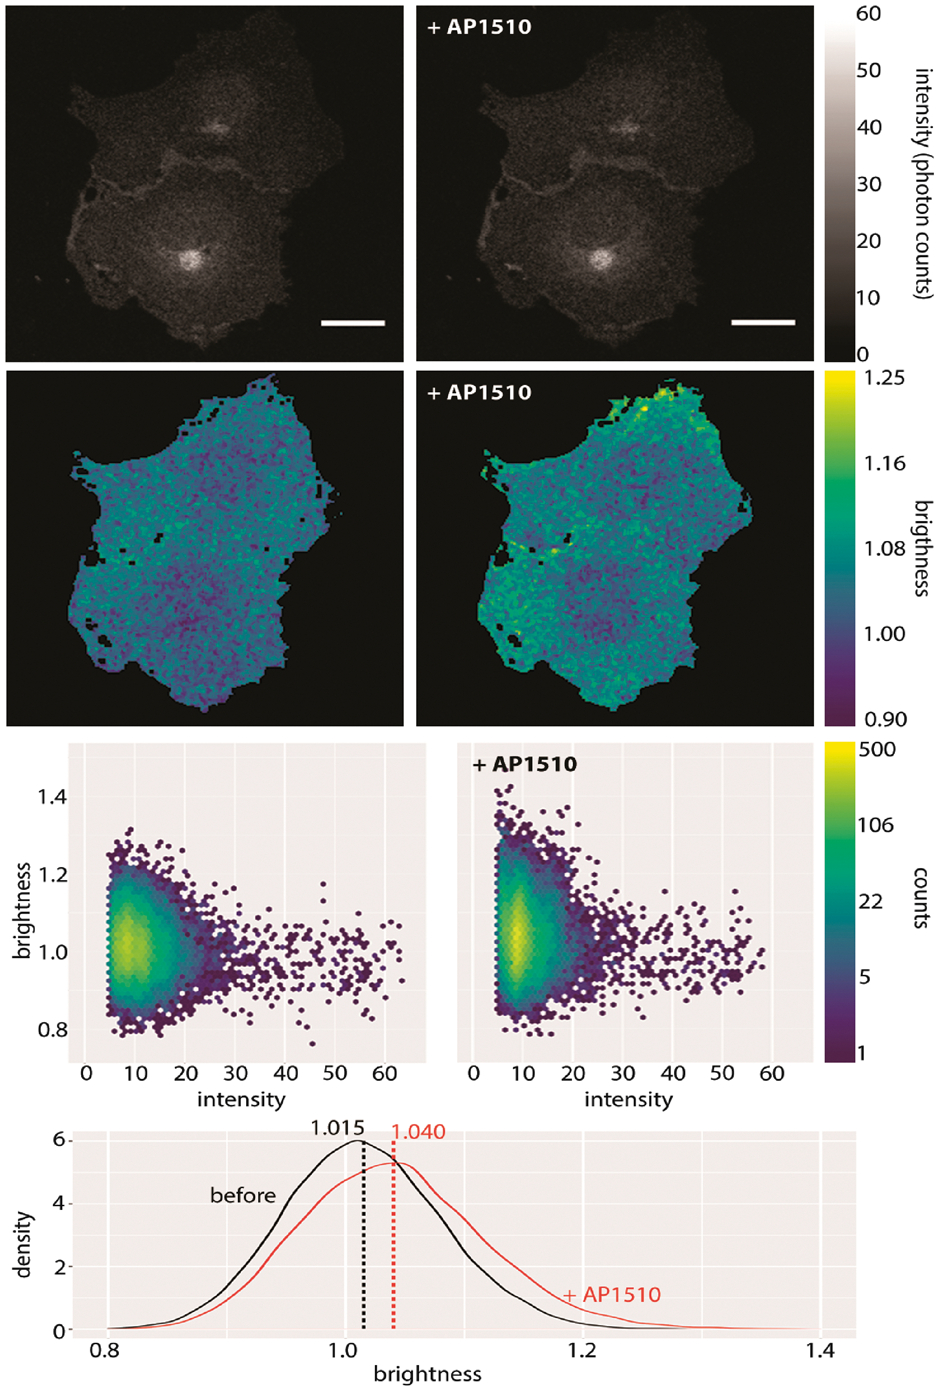
\includegraphics[width=1\linewidth]{/home/travis/build/rorynolan/phdthesis/img/nandb-fig} \hfill{}

\caption{mClover-labelled myristoylated FKBP12 before and
after application of 50nM AP1510. Shown here are intensity (first row),
brightness (second row), a plot of intensity versus brightness (third
row) and brightness histograms (fourth row). Notice how the change in
brightness upon addition of the drug is seen most clearly by comparing
the brightness histograms. The vertical lines in the histogram plot show
the means of those histograms. Brightness here refers to B. Scale bar 20
\(\mu\)m. \citep{nandb}}\label{fig:nandb-fig}
\end{figure}

\subsection{Visualization of bleaching correction on real
data}\label{visualization-of-bleaching-correction-on-real-data}

That publication also includes a visualization of bleaching correction
on real data. Figure \ref{fig:bleachvis1} shows this, comparing the
choice of \(\tau=10\) with the automatic detrending algorithm, which
chooses an appropriate \(\tau\) based on the data. It is evident that
both \(\tau=10\) and the automatic choice of \(\tau\) give the corrected
intensity profile a stationary mean (both the red and green series start
and end at \(\approx 11\)), however the \(\tau = 10\) correction (red
line) also has a much decreased variance compared to the auto \(\tau\)
line (green), which is bad; the \(\tau = 10\) line is removing local
variation, which is exactly what we're trying to avoid.




\begin{figure}

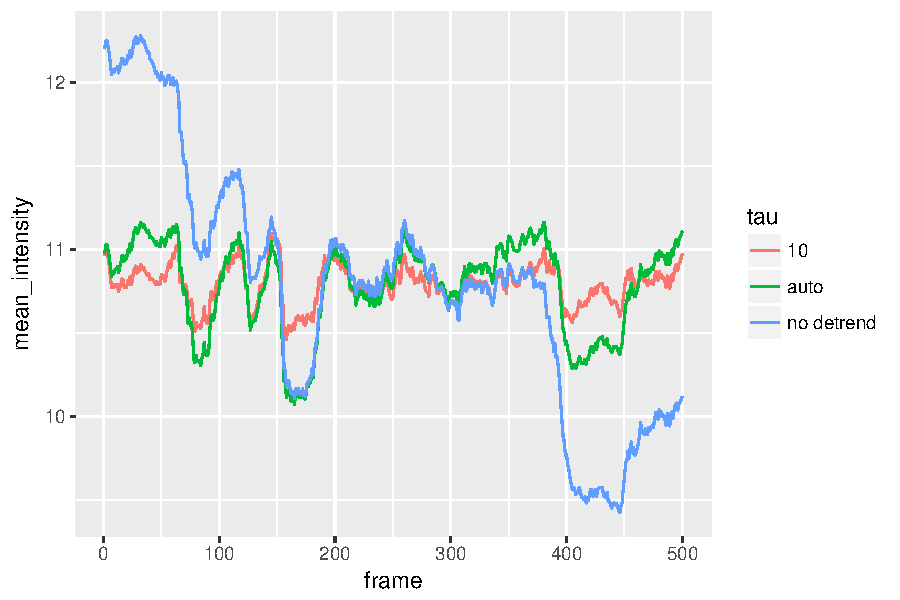
\includegraphics[width=1\linewidth]{/home/travis/build/rorynolan/phdthesis/img/bleachvis1} \hfill{}

\caption{Real data image series mean intensity profile
with bleaching correction with \(\tau = 10\) and auto \(\tau\).}\label{fig:bleachvis1}
\end{figure}

\section{\texorpdfstring{\emph{In vitro} number and
brightness}{In vitro number and brightness}}\label{in-vitro-number-and-brightness}

\subsection{Introduction}\label{introduction-1}

In our research group, we believe that the most practical quantitative
method for measuring homo-dimerization \emph{in vivo} and \emph{in
vitro} is N\&B \citep{NB} because it is calibration-free and does not
require specialized instrumentation. There are many examples of the
application of N\&B \emph{in vivo} (the original N\&B paper has over 250
citations, most of which are \emph{in vivo} applications) but none
\emph{in vitro}. Hence, we published a protocol \citep{JOVE} detailing
how N\&B can be applied \emph{in vitro}. This time, we used FKBP12F36V
which is an FKBP mutant with a new dimerizing drug AP20187 (known
colloquially as the \emph{BB dimerizer}); this pair is designed to have
better specificity than the original \citep{Clackson}.

\subsection{Experimental results and
discussion}\label{experimental-results-and-discussion-1}

In this experiment, the FKBP12F36V was labelled with mVenus. We found
that the brightness doubled from \(\epsilon = 0.005\) to
\(\epsilon = 0.010\) upon addition of the drug. See figure
\ref{fig:jove}. This analysis was done with exponential smoothing
detrending with automatically chosen parameter \(\tau\). Without
detrending, the pre-BB brightness was calculated as
\(\epsilon = 0.026\), showing that detrending is absolutely necessary
and that neglecting this step can lead to nonsensical results.





\begin{figure}

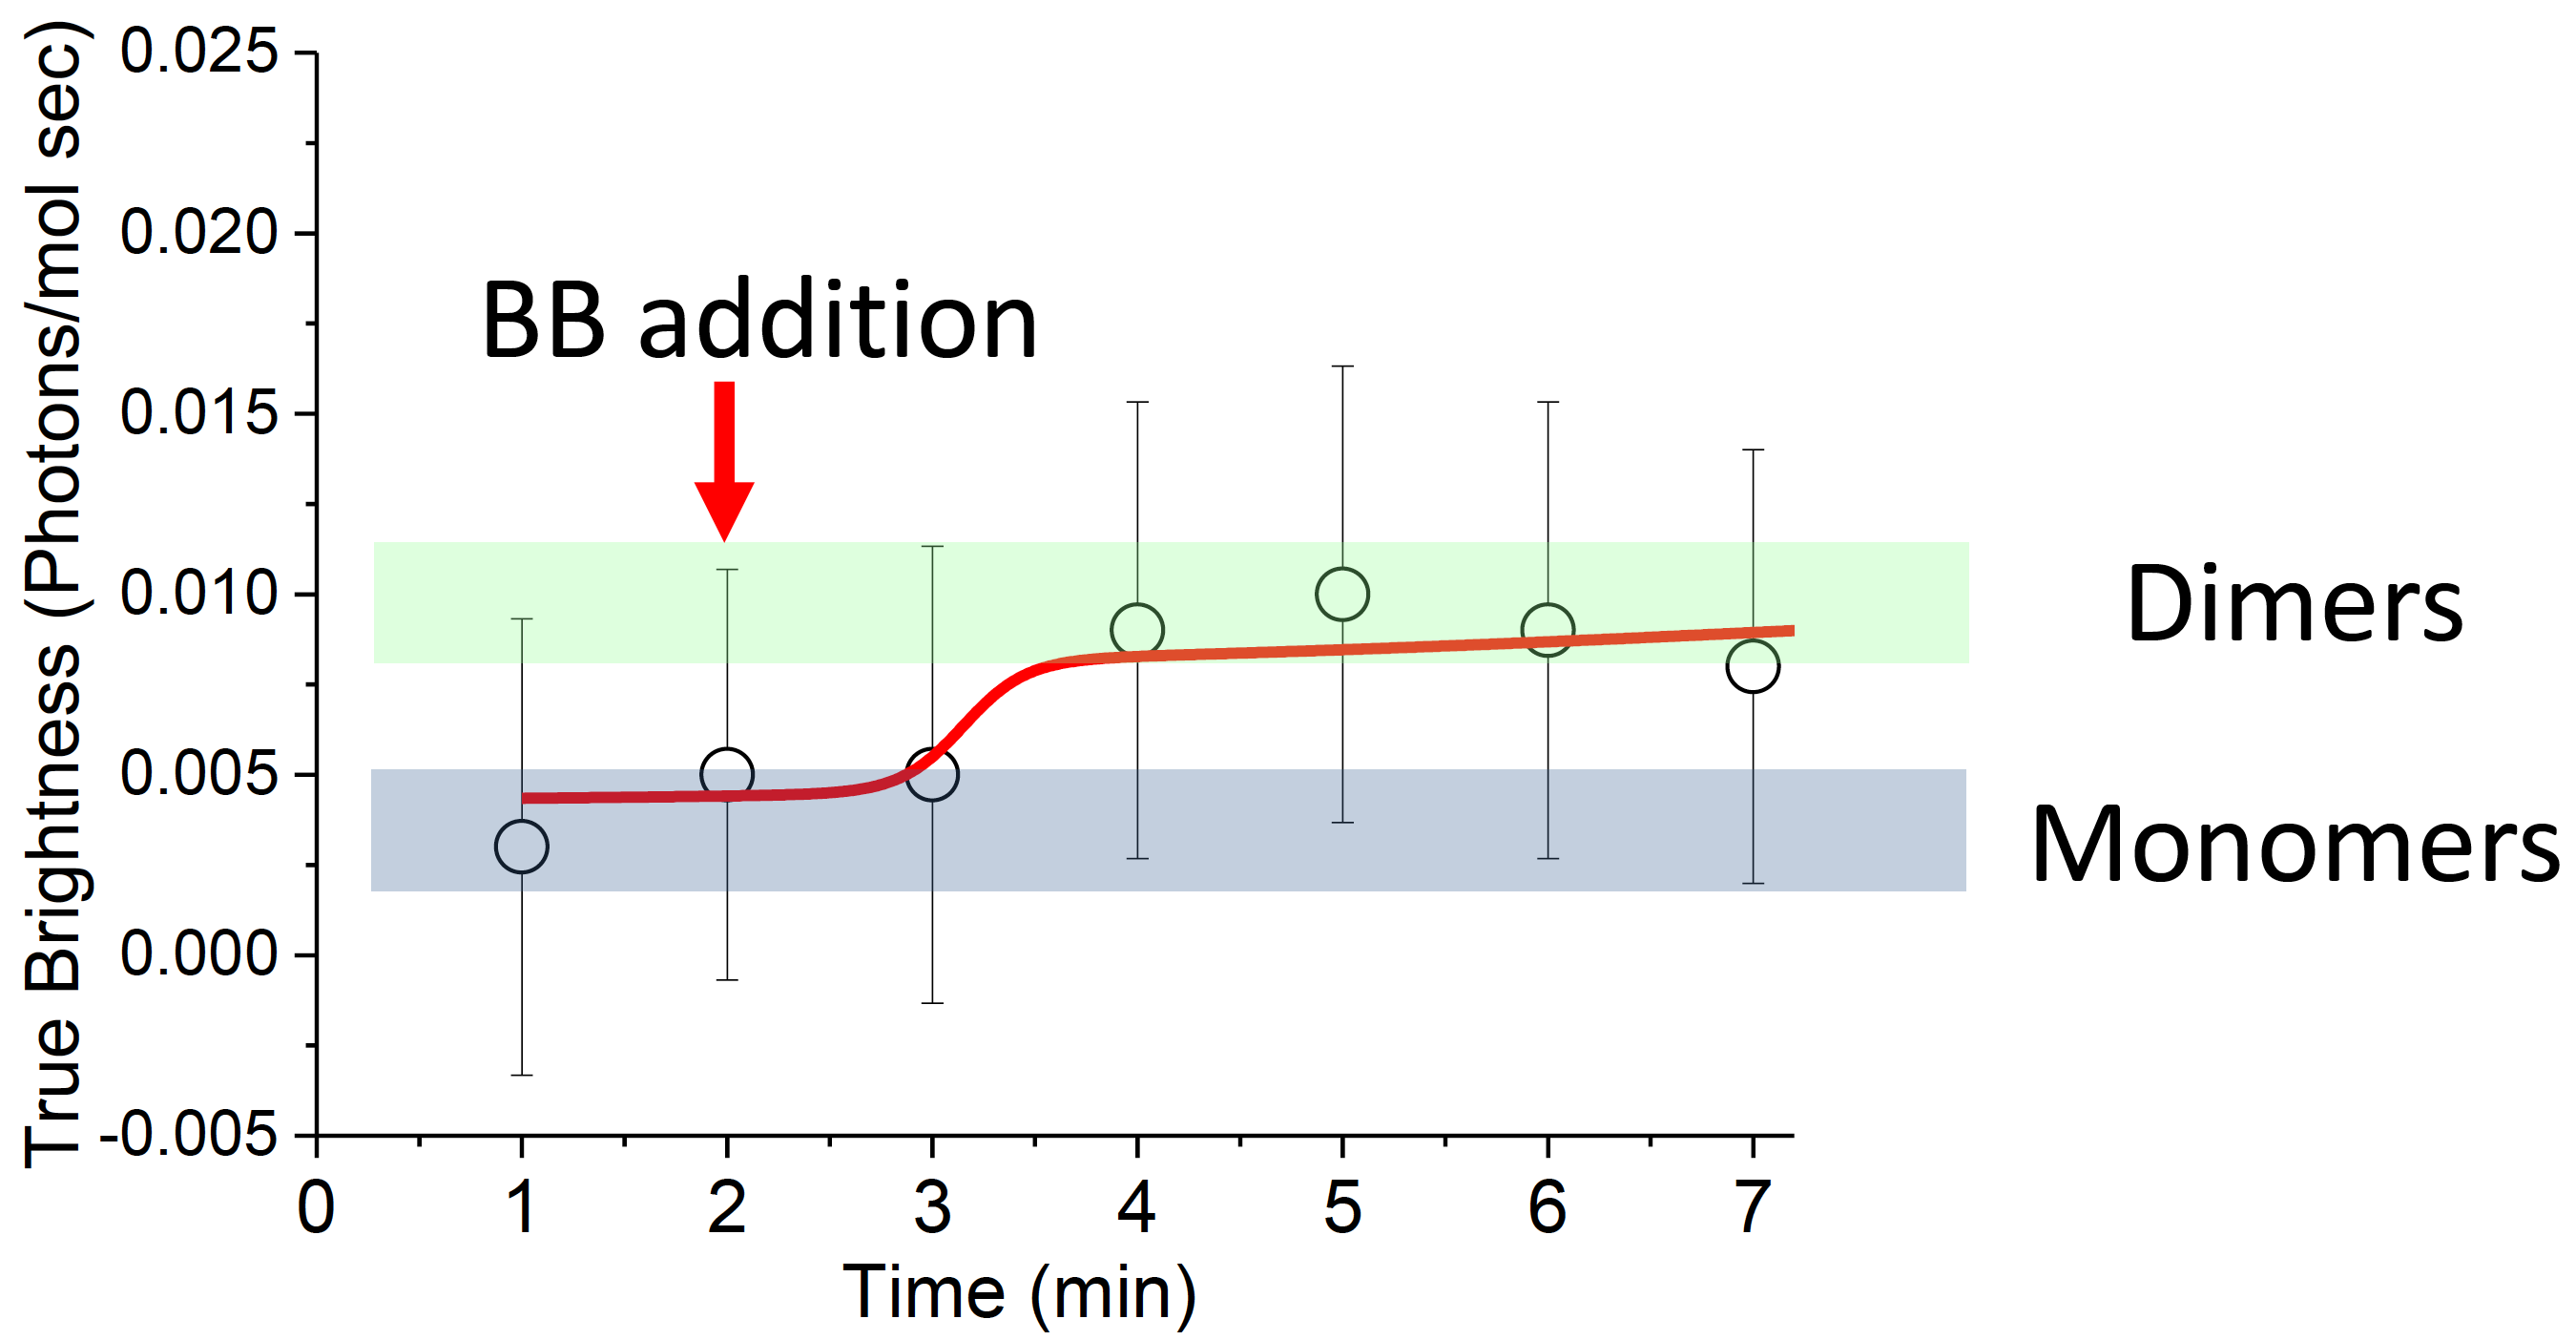
\includegraphics[width=1\linewidth]{/home/travis/build/rorynolan/phdthesis/img/jove-dimerization} \hfill{}

\caption{Dimerization of FKBP12F36V upon BB addition is seen
by a brightness doubling from \(\epsilon = 0.005\) to
\(\epsilon = 0.010\) over a period of minutes.}\label{fig:jove}
\end{figure}

\BeginKnitrBlock{remark}
\iffalse{} {Remark. } \fi{} This paper also included an important
correction to the equation for brightness \(\epsilon\) when analog
equipment is used. The correct equation is

\begin{equation}
\epsilon = \frac{\sigma^2 - \sigma_0^2}{S(\langle I \rangle - \text{ offset})}
\label{eq:dalaleq}
\end{equation}

The \(S\) in the denominator was omitted in the original paper
\citep{Dalal} and this error was reproduced in our N\&B review
\citep{NBreview}.
\EndKnitrBlock{remark}

\section{HIV-1 receptor
stoichiometry}\label{hiv-1-receptor-stoichiometry}

\subsection{Introduction}\label{introduction-2}

\subsubsection{HIV-1 cell entry}\label{hiv-1-cell-entry}

HIV-1 infects many cell types (e.g.~CD4 T cells, macrophages, dendritic
cells) and has different modes of entry for each cell type and indeed
possible more than one mode of entry in any given cell type
\citep{Jakobsdottir}. Endocytosis is thought to be a common entry route
\citep{Miyauchi}, particularly in macrophages \citep{Marechal} and
Dendritic cells \citep{Mnager}. In CD4 T cells, HIV-1 has been shown to
fuse at the plasma membrane without needing endocytosis \citep{Herold}.

Entry of HIV into any cell involves the initial binding of the CD4
receptor on that cell by the HIV-1 virus. Subsequently, a co-receptor
(often CCR5 or CXCR4) is used in the fusion process
\citep{Jakobsdottir}. The question of how many receptors and
co-receptors are required to facilitate fusion (the \emph{stoichiometry}
of the interaction of HIV-1 with its receptor and co-receptor, possibly
different for different cell types) had not been answered.

\subsubsection{The use of number and brightness to study HIV-1 cell
entry}\label{the-use-of-number-and-brightness-to-study-hiv-1-cell-entry}

Our main motivation for studying N\&B in the first place was that we
thought it was a valuable method to study the process of HIV-1 fusion in
live cells. N\&B was first used in our research group to study the
oligomeric state of dynamin at the HIV-1 fusion pore in TZM-bl cells
\citep{DanDynamin}. This study concluded that dynamin-2 stabilizes the
HIV-1 fusion pore with a low oligomeric state.

Following on from this, we wanted to study the stoichiometry of the
interaction of HIV-1 with its receptor (CD4) and co-receptor (CCR5 or
CXCR4) upon the engagement of the virus with the cell and to follow this
interaction stoichiometry up to the point of fusion. See figure
\ref{fig:HIVStoichiometrySetup}.

\begin{quote}
Entry of HIV-1 into a host cell requires an initial interaction between
the viral-envelope glycoprotein spike complex---Env---with cell surface
displayed CD4 and co receptors \citep{Jakobsdottir}. Although structural
studies have revealed the intra-molecular basis for CD4 receptor and
CXCR4/CCR5 co-receptor-induced conformational changes to the HIV-1 Env
during host cell entry \citep{Ozorowski}, little is known about how the
inter-molecular dynamics and stoichiometry of this process culminates in
fusion with the host cell membrane in live cells \citep{Brandenberg}.
This is due to the difficulty of working with live cells and the lack of
temporal resolution of the techniques commonly employed
(i.e.~crystallography and cryo-EM).

--- \citet{HIVstoichiometry}
\end{quote}









\begin{figure}

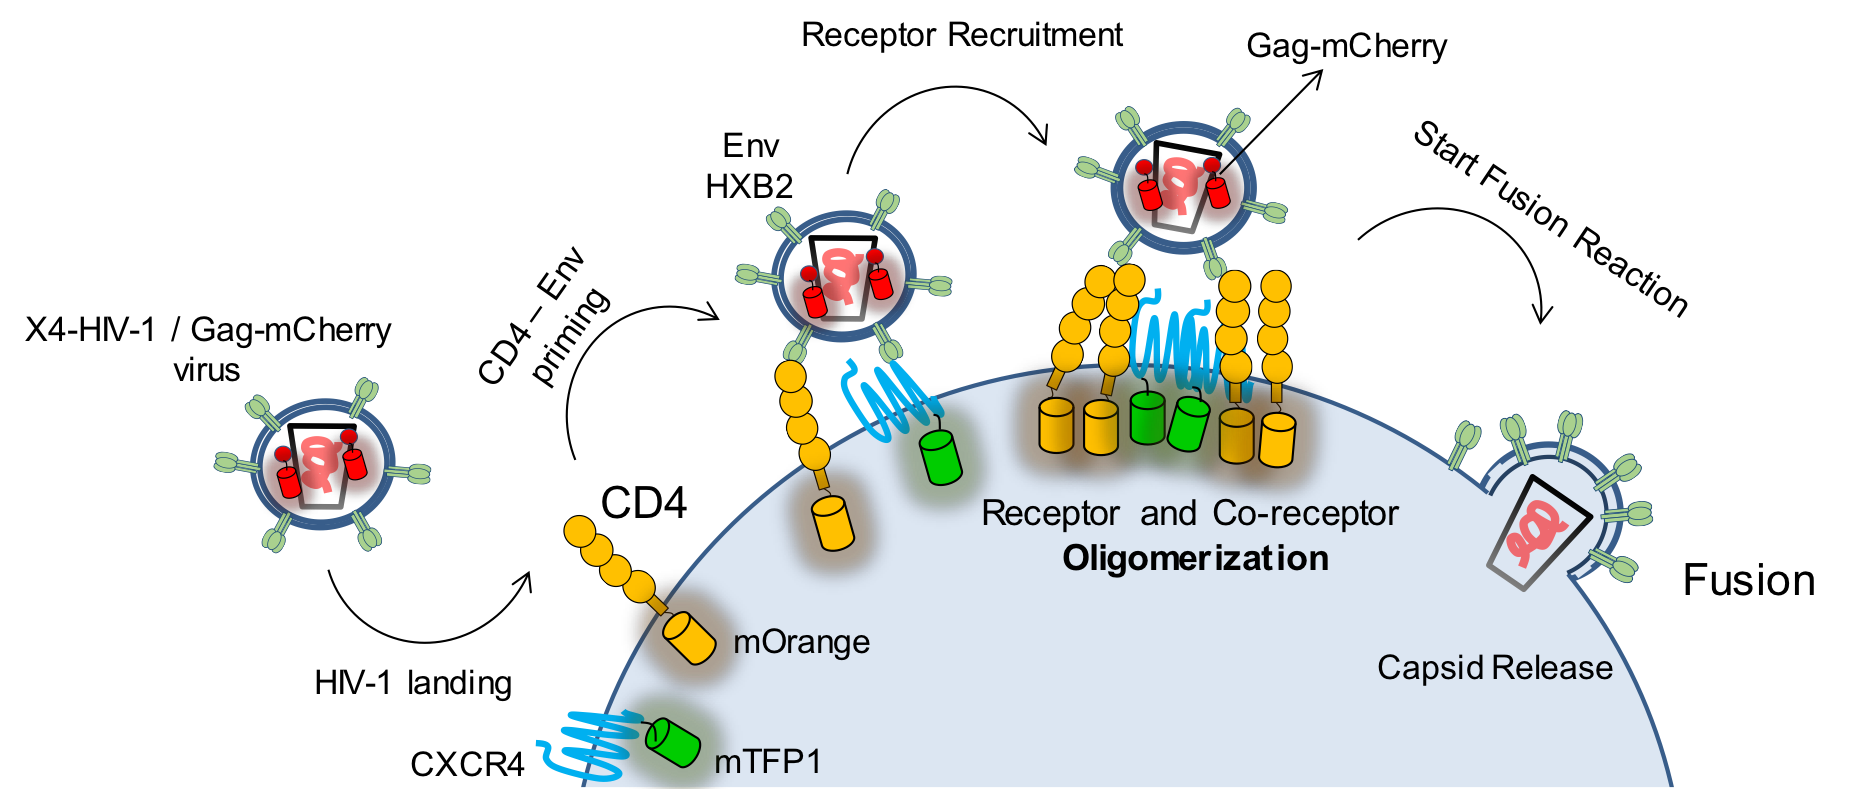
\includegraphics[width=1\linewidth]{/home/travis/build/rorynolan/phdthesis/img/HIVStoichiometrySetup} \hfill{}

\caption{The HIV-1 envelope glycoprotein Env
must bind the receptor (CD4) and form a complex with the co-receptor
(CXCR4 or CCR5, this figure shows an X4-tropic virus and co-receptor) to
initiate the fusion process. Labeling the viral Gag protein with
mCherry, the receptor with mTFP1 and the co-receptor with mOrange, it is
possible to follow these three players in the fusion reaction and to
quantify their interaction.}\label{fig:HIVStoichiometrySetup}
\end{figure}

We saw N\&B as the ideal technique to probe this stoichiometry
temporally. With our microscope, we could acquire 100 frames per 1.7
minutes, therefore, using each consecutive sequence of 100 frames to
create a brightness image, we could obtain 1 brightness image every 1.7
minutes and use this to calculate this temporal stoichiometry.

\subsection{Experimental setup}\label{experimental-setup}

Receptor (CD4) and co-receptor (CXCR4 or CCR5) were labelled in Cos7
cells. Virus was added at time \(t=0\) and imaging proceeded for a
number of minutes at 100 frames per 1.7 minutes. Alternating laser
excitation (ALEX, \citet{ALEX}) was used to eliminate the possibility of
channel bleed-through. See figure \ref{fig:HIVStoichiometryIntensity}.





\begin{figure}

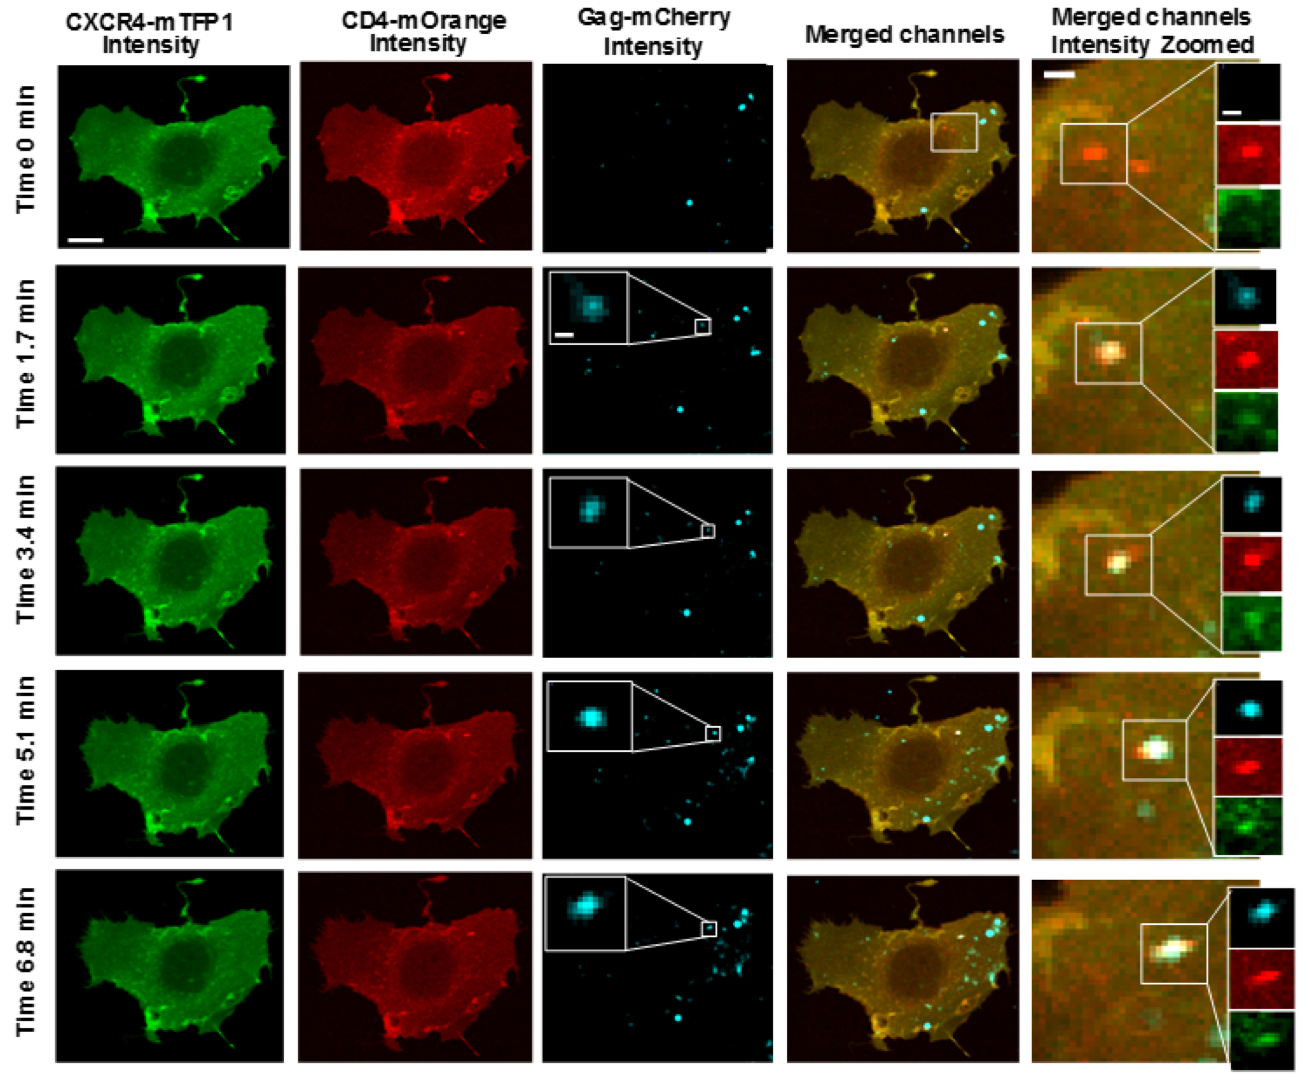
\includegraphics[width=1\linewidth]{/home/travis/build/rorynolan/phdthesis/img/HIVStoichiometryIntensity} \hfill{}

\caption{Intensity images from the virus,
receptor and co-receptor. Every 100\textsuperscript{th} frame is shown.
A virus which lands at \(t \approx 1.7\) minutes is highlighted.}\label{fig:HIVStoichiometryIntensity}
\end{figure}

\subsection{Analysis}\label{analysis}

The virus channel was used to locate the virus at a given point in time.
The receptor and co-receptor were used to calculate brightness and
cross-correlated brightness every 100 frames (every 1.7 min). The
brightness was used to determine the number of receptor and co-receptor
units involved in a complex. The cross-correlated brightness was used to
delimit whether or not the receptor and co-receptor units were together
in the \emph{same} complex. See figure
\ref{fig:HIVStoichiometryAnalysis}, this is the corresponding brightness
and cross-correlated brightness image of figure
\ref{fig:HIVStoichiometryIntensity}. Notice that once the virus lands,
the oligomeric state of the receptor and co-receptor increases. We also
see significant positive cross-correlated brightness in this area,
indicating that the virus has triggered a complex of receptor and
co-receptor.





\begin{figure}

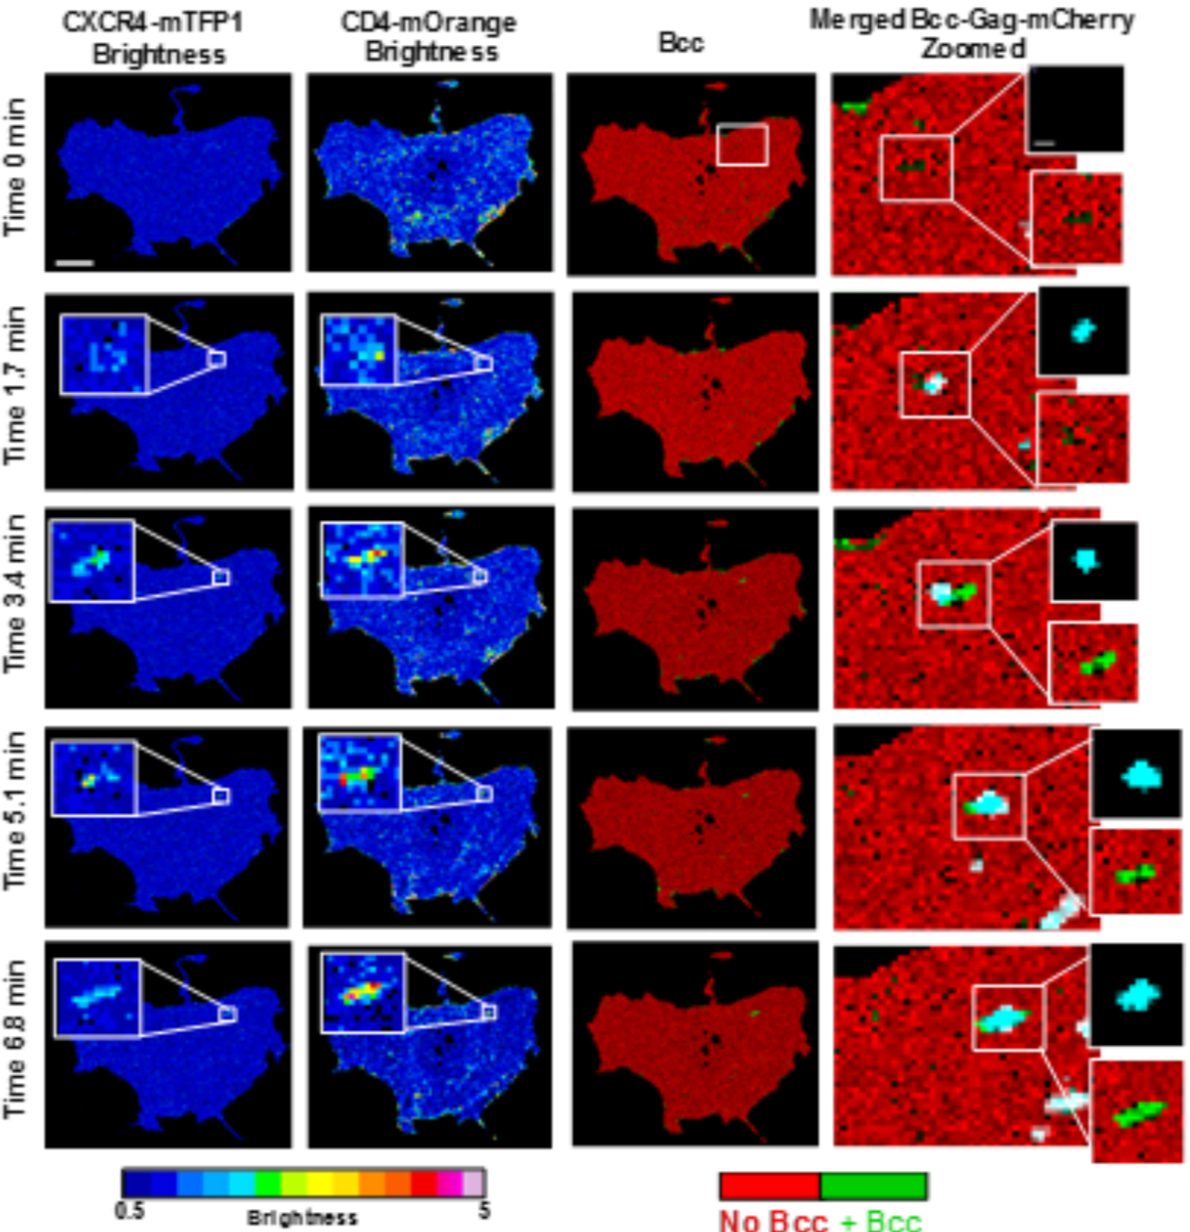
\includegraphics[width=1\linewidth]{/home/travis/build/rorynolan/phdthesis/img/HIVStoichiometryAnalysis} \hfill{}

\caption{Brightness images of receptor and
co-receptor and cross-correlated brightness image of the interaction
between the two.}\label{fig:HIVStoichiometryAnalysis}
\end{figure}

\subsection{Results}\label{results}

Figure \ref{fig:HIVStoichiometryPlots} shows the results of the analysis
detailed in figures \ref{fig:HIVStoichiometryIntensity} and
\ref{fig:HIVStoichiometryAnalysis} for \(n=10\) cases where virus
triggered receptor and co-receptor complexes in the X4-tropic setting
and \(n=12\) in the R5-tropic setting. A three-step pre-fusion process
is hypothesized for each.






\begin{figure}

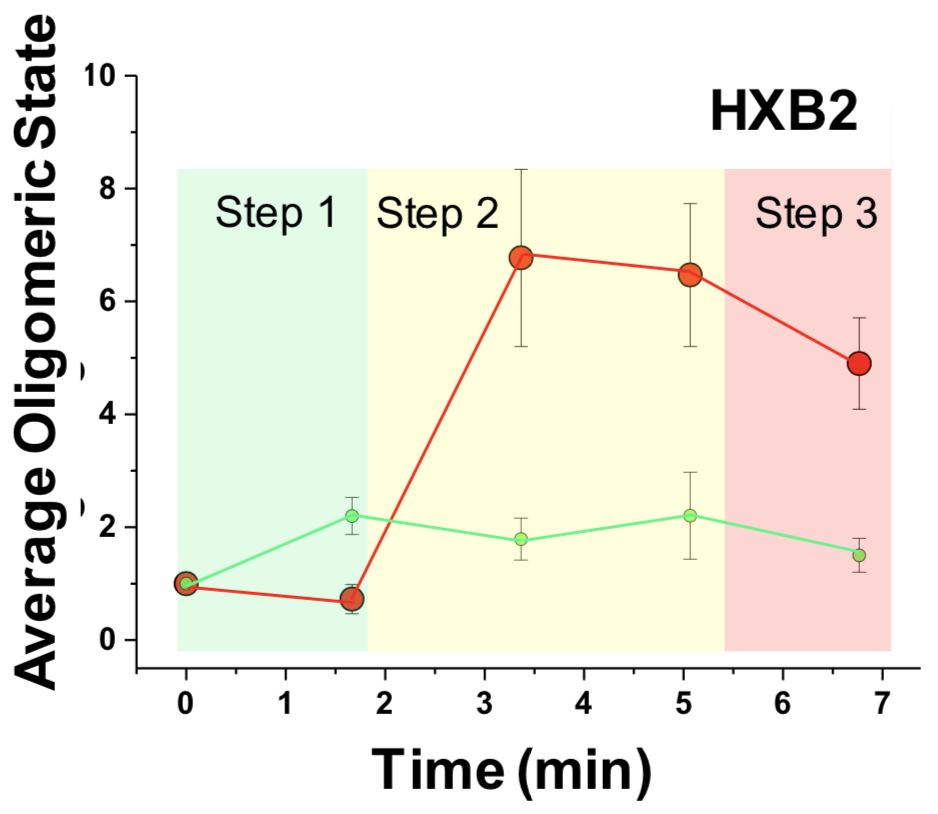
\includegraphics[width=0.47\linewidth]{/home/travis/build/rorynolan/phdthesis/img/X4plot} 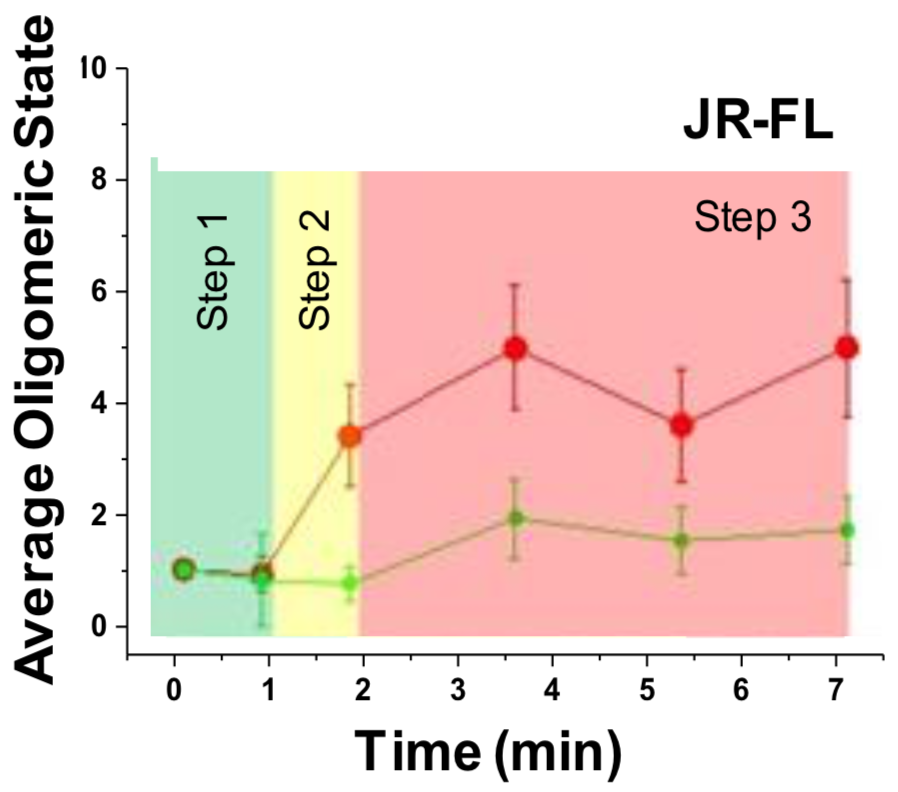
\includegraphics[width=0.47\linewidth]{/home/travis/build/rorynolan/phdthesis/img/R5plot} \hfill{}

\caption{Number of receptor and co-receptor
units involved in complexes with virus over time, obtained by brightness
analysis. Left panel: HIV\textsubscript{HXB2}. Right panel:
HIV\textsubscript{JR-FL}.}\label{fig:HIVStoichiometryPlots}
\end{figure}

\begin{quote}
Our studies support a dynamic three step model for both HIVHXB2 and
HIVJR-FL (figure \ref{fig:HIVStoichiometryStructure}). For X4 tropic
virions, Env -- CD4 interactions induce CXCR4 dimerization, CD4 then
engages with two Env (shown by 3 color TIRF-dSTORM microscopy) to
generate a hexamer that might serve as a scaffold to stabilise a final 4
CD4 -- 1/2 CXCR4 conformation, with a single Env. We speculate that for
HIVHXB2, step 2 is crucial to culminate the fusion reaction and there
could be an anchoring domain and a fusion domain that undergoes gp120
disassembly leading to 6 helix bundle formation. For R5 tropic virions,
Env -- CD4 interactions form a the previously described asymmetric
pre-hairpin intermediate \citep{Munro} \citep{DoKwon} \citep{Ma};
following binding and oligomerisation of 2 additional CD4 molecules with
concomitant CCR5 dimerization. After this, the secondary intermediate
leads to the final fusion competent complex with a total of 4±0.3 CD4,
2±0.3 CCR5 and 1 JR-FL Env.
\end{quote}

\begin{quote}
Our data indicate that both HXB2 Env and JR-FL Env start with an
asymmetric intermediate bound to a single CD4, as previously
suggested27. Our models also support the existence of important
differences in the entry mechanisms of X4 and R5 strains. In the X4
strains, CXCR4 dimerization \citep{Tan} {[}Qin{]} occurs prior to CD4
hexamer formation and following initial Env -- CD4 recognition
\citep{Liu}. For R5 tropic JR-FL, CCR5 dimerization \citep{Qin} occurs
after Env-CD4 complexation and recruitment of two additional CD4
molecules \citep{Wu} around the complex.

--- \citet{HIVstoichiometry}
\end{quote}

For the X4 and R5-tropic case, structural modelling of the hypothesis
has been done. See figure \ref{fig:HIVStoichiometryStructure}.







\begin{figure}

\includegraphics[width=1\linewidth]{/home/travis/build/rorynolan/phdthesis/img/HIVStoichiometryStructure} \hfill{}

\caption{The HIV-1 JR-FL Env glycoprotein
(blue) (PDB ID: 4ZMJ) is present as a trimer on the mature virion. b,
Time-resolved stoichiometry pre-fusion reaction for CXCR4-CD4 (red dots)
induced by HIVHXB2--Gag-iCherry virions. (gp120: light blue, gp41: dark
blue, CD4: orange, CXCR4: green, b12: yellow)}\label{fig:HIVStoichiometryStructure}
\end{figure}

\subsection{Conclusion}\label{conclusion}

Time-resolved N\&B enabled us to answer questions about the interaction
between the HIV-1 virus and its receptor and co-receptor in live cells
which up to now could not be answered. Being able to correctly correct
for bleaching is crucial for reliable N\&B analysis, so the development
of these new algorithms was crucial to this study.

\chapter{Discussion}\label{discussion}

\section{Fluorescence fluctuation
spectroscopy}\label{fluorescence-fluctuation-spectroscopy}

Even with photon-counting detectors, FFS is a difficult technique. There
are many pitfalls: the acquisition settings (dwell time and frame rate)
must be correct and the correct settings for these parameters depend on
the residence time \(\tau_D\) of the protein of interest, which is
non-trivial to measure. The acquired data must be checked to ensure
there is not an excess of photobleaching and if there is not, there will
inevitably still be some bleaching, so this must be corrected for. Until
now, it was practically impossible to perform this correction correctly,
because all methods required the user to select a vital correction
parameter (\(\tau\) or \(l\)) without providing any instructions as to
how the parameter should be chosen. I have now solved this problem such
that now image series can be safely detrended by novice users, as this
parameter is chosen for them in the background. Now, detrending an image
\texttt{img.tif} with the \emph{Robin Hood} method is as simple as
typing the command \texttt{img\_detrend\_rh("img.tif")} in my software.
This should make FFS techniques safer and easier to use, opening FFS
techniques up to more users, however the expertise required is still
such that FFS may struggle to expand from the domain of microscopy and
biophysics into a more commonly used biological technique.

\section{The evolution of detrending
algorithms}\label{the-evolution-of-detrending-algorithms}

Previously, FFS detrending methods were based on smoothing methods taken
from the field of time-series analysis. The fact that these smoothing
methods required a choice of smoothing parameter was ignored by sticking
to the arbitrary choice of \(l=10\) for this parameter.

My work in investigating the significance of this smoothing parameter
found that this arbitrary choice was totally incorrect. The use of
simulated image series and the fact that immobile particles have
brightness \(B=1\) opened up a means of solving for the correct choice
of this parameter without the need for user input. This was the first
set of \emph{automatic detrending} methods, whereby to detrend, the
users task was a simple as clicking a \texttt{detrend} button.

Still, using smoothing approaches to detrend low-intensity data is
problematic because it involves approximating very discrete time series
with continuous functions; this is unwise and unnecessary. The
\emph{Robin Hood} idea of giving photon counts directly from one pixel
to another in an image series circumvents the need for smoothing. The
detrending process can be simplified from
\(\mathbb{N}_0 \rightarrow \mathbb{R} \rightarrow \mathbb{N}_0\) to
\(\mathbb{N}_0 \rightarrow \mathbb{N}_0\). Conveniently, the automatic
approach used in the smoothing approaches to detrending can readily be
extended to \emph{Robin Hood} detrending.

There are no obvious caveats to the \emph{Robin Hood} bleaching
correction method and thus no more work is needed on its theory.
However, it is vital to bear in mind that one should always try to avoid
the source of error in the first place rather than rely on correction
methods.

\section{Applications of the new detrending
techniques}\label{applications-of-the-new-detrending-techniques}

\subsection{FKBP}\label{fkbp}

The FKBP applications of these detrending techniques in Cos-7 cells
\citep{nandb} and in-vitro were mainly to demonstrate that N\&B used
with these detrending techniques is a reliable method to measure
oligomerization. The in vitro study \citep{JOVE} was particularly
interesting because it was the first in vitro application of number and
brightness.

\subsection{HIV-1 receptor
stoichiometry}\label{hiv-1-receptor-stoichiometry-1}

The study of HIV-1 receptor stoichiometry \citep{HIVstoichiometry} is a
\emph{real-life} application of N\&B and ccN\&B, made possible by the
automatic detrending algorithm. We have shown that this kind of
fine-grained information about the process of HIV-1 fusion can be
measured on a temporal basis in live cells. Whilst this alone is very
exciting, it paves the way for similar studies to be done with HIV-1 and
different cell types and indeed for other virus fusion processes to be
probed in this way.

\subsection{Multiplexing with structural
biology}\label{multiplexing-with-structural-biology}

Our collaboration with structural biologists \citep{HIVstoichiometry} is
a demonstration of how live cell fluorescence microscopy and structural
biology can be complementary. The sub-molecular insight from structural
biology is not available from live cell fluorescence microscopy, while
the dynamic information from live cell fluorescence microscopy cannot be
gotten from structural biology.

\subsection{Fluorescence fluctuation
spectroscopy}\label{fluorescence-fluctuation-spectroscopy-1}

FFS has many applications. Indeed the original N\&B paper \citep{NB}
alone has over 250 citations. All of these and future FFS studies
require correct detrending to be reliable. \emph{Robin Hood} detrending
is the answer for this. A major challenge will be making \emph{Robin
Hood} visible, available and easy to use for the community. This means
that the algorithm must be peer-reviewed, made available in all of the
major free imaging softwares (ImageJ, python, R) and very well
documented: a good manual is essential with any software package.

\chapter{Future plans}\label{future-plans}

\section{Robin Hood publication}\label{robin-hood-publication}

The \emph{Robin Hood} algorithm is already incorporated in the R package
\texttt{detrendr} but it hasn't been published or peer-reviewed. Getting
this done is my top priority.

\section{\texorpdfstring{Translate software to
\emph{ImageJ}}{Translate software to ImageJ}}\label{translate-software-to-imagej}

Whilst I really like R, the fluorescence community does not use it,
which has been a major barrier to the use of my algorithms. I will code
my detrending algorithms as \emph{ImageJ} plugins and also as python
modules so that more of the community have easy access to them.

\section{Study real data bleaching profiles with
simulations}\label{mimic}

It was mentioned in section \ref{detrend-compare} that it would be
possible to study the effect of real bleaching as opposed to simulated
ideal bleaching and why it is more necessary to detrend in the real data
case by mimicking real bleaching profiles with simulations. This is
something I would like to do. It would be difficult because it would
require the collection and cataloging of a diverse set of real data
bleaching profiles from various biological samples. This would be the
bottleneck because I have already written the simulation and analysis
pipelines.

\section{Compare FRET with FCS}\label{compare-fret-with-fcs}

I have the idea that when the question ``Do these proteins interact?''
is answered by Forster resonance energy transfer (FRET, \citet{Frster}),
it should also be answerable by FCS. I would like to try to reproduce
some standard FRET results with FCS. I am particularly interested to
find out if there are instances where one technique succeeds and the
other fails and why this might be. For example, it might be possible
that for a given interacting pair of proteins, it is impossible to label
them such that the FRET couple is close enough for FRET to be detected,
but that this interaction is detectable by FCS. These techniques have
been compared before \citep{Sahoo}, but not by trying to reproduce
previous work. In addition, attempts by new groups to reproduce work
that is accepted in the literature are always interesting
\citep{Baker2016}.

\bibliography{book.bib,packages.bib,papers.bib,webpages.bib}


\end{document}
